%% 
%% Copyright 2007-2025 Elsevier Ltd
%% 
%% This file is part of the 'Elsarticle Bundle'.
%% ---------------------------------------------
%% 
%% It may be distributed under the conditions of the LaTeX Project Public
%% License, either version 1.3 of this license or (at your option) any
%% later version.  The latest version of this license is in
%%    http://www.latex-project.org/lppl.txt
%% and version 1.3 or later is part of all distributions of LaTeX
%% version 1999/12/01 or later.
%% 
%% The list of all files belonging to the 'Elsarticle Bundle' is
%% given in the file `manifest.txt'.
%% 
%% Template article for Elsevier's document class `elsarticle'
%% with harvard style bibliographic references

\documentclass[preprint,12pt,authoryear]{elsarticle}

%% Use the option review to obtain double line spacing
%% \documentclass[authoryear,preprint,review,12pt]{elsarticle}

%% Use the options 1p,twocolumn; 3p; 3p,twocolumn; 5p; or 5p,twocolumn
%% for a journal layout:
%% \documentclass[final,1p,times,authoryear]{elsarticle}
%% \documentclass[final,1p,times,twocolumn,authoryear]{elsarticle}
%% \documentclass[final,3p,times,authoryear]{elsarticle}
%% \documentclass[final,3p,times,twocolumn,authoryear]{elsarticle}
%% \documentclass[final,5p,times,authoryear]{elsarticle}
%% \documentclass[final,5p,times,twocolumn,authoryear]{elsarticle}

%% For including figures, graphicx.sty has been loaded in
%% elsarticle.cls. If you prefer to use the old commands
%% please give \usepackage{epsfig}

\usepackage{amssymb}
\usepackage{amsmath}
\usepackage{orcidlink}
\usepackage{url}
\usepackage{float}
\usepackage{booktabs}
\usepackage{longtable}
\usepackage{hyperref} 
\usepackage{graphicx}
\usepackage{multirow}
\hypersetup{
    colorlinks=false,
    linkcolor=blue,
    filecolor=magenta,      
    urlcolor=cyan,
    pdftitle={Your Document Title},
    pdfpagemode=FullScreen,
}
%% The amsthm package provides extended theorem environments
%% \usepackage{amsthm}

%% The lineno packages adds line numbers. Start line numbering with
%% \begin{linenumbers}, end it with \end{linenumbers}. Or switch it on
%% for the whole article with \linenumbers.
%% \usepackage{lineno}
\journal{Computational Toxicology}
\begin{document}
\begin{frontmatter}
\title{A Multi-Route Permeability-Limited Physiologically-Based Kinetic Model for Perfluorooctanoic Acid in Male and Female Rats} 
\author{Paraskevi Papakyriakopoulou\fnref{label2}\orcidlink{0000-0003-0566-0713}}
\author{Periklis Tsiros\fnref{label2}\orcidlink{0000-0002-7179-8086}}

\author{Vasileios Minadakis\orcidlink{0009-0004-2521-4432} }

\author{Haralambos Sarimveis\corref{cor1}\orcidlink{0000-0002-8607-9965}}
\ead{hsarimv@central.ntua.gr}
\fntext[label2]{These authors contributed equally }
\cortext[cor1]{Corresponding author}
\affiliation{organization={School of Chemical Engineering, National Technical University of Athens},
addressline={9 Heroon Polytechneiou Street}, 
            city={Zografou},
            postcode={15780}, 
            state={Attiki},
            country={Greece}}
\begin{abstract}
Per- and polyfluoroalkyl substances (PFAS) are persistent synthetic chemicals extensively used in industrial applications and consumer products .  Perfluorooctanoic acid (PFOA) being one of the most studied congeners, has been detected in up to $99\%$ of individuals in the U.S. population and is linked to various adverse health effects. While ingestion of contaminated food and water is the primary exposure route, inhalation also contributes to human PFOA intake, particularly in occupational settings. In this context, a physiologically based kinetic (PBK) modelling offers a mechanistic framework for simulating the absorption, distribution, and excretion of PFOA across various organs and tissues and understanding key processes that affect its internal disposition. A comprehensive full-body structure, including 17 distinct tissue compartments was developed to describe the biodistribution of PFOA in male and female rats after intravenous administration, oral exposure and inhalation. Part of the effort focused on determining if vitro parameterisation is sufficient to develop a reliable model.. The model builds upon and extends previous permeability-limited modelling attempts using a middle-out approach, with parameterization through both \textit{in vitro} and in vivo data. Extensive validation with multiple doses showed good agreement between predicted and observed concentrations in plasma, tissues, and excreta. Sensitivity analysis revealed that parameters related to protein binding were the most influential across all compartments. This work offers valuable insights into the impact of protein binding, passive diffusion and facilitated transport in the observed profiles of male and female rats across various exposure routes.

\end{abstract}

%%Graphical abstract
\begin{graphicalabstract}
%
\includegraphics{grabs}
\end{graphicalabstract}

%%Research highlights
\begin{highlights}
\item Research highlight 1
\item Research highlight 2
\end{highlights}

%% Keywords
\begin{keyword}
perfluorooctanoic acid \sep physiologically-based kinetic model \sep  inhalation \sep  toxicokinetics \sep  rat 
\end{keyword}
\end{frontmatter}
\newpage
\section{Introduction}
\label{PFOA_intro}
Per- and polyfluoroalkyl substances (PFAS) are synthetic chemicals, extensively utilized in industry applications and consumer products since the 1950s. They are found in nonstick cookware, stain resistant fabrics and carpets, some cosmetics and aqueous film-forming firefighting foams \citep{gluge_2020}. These chemicals are characterized by high persistence in extreme temperatures and amphiphilic properties allowing for use in both water and oil repellent coatings \citep{cao_2021}. 

Within the PFAS class of chemicals, perfluorooctanoic acid (PFOA) is among the most extensively studied congeners.  It resists biodegradation, leading to bioaccumulation in the food chain and in the human body over time \citep{peritore_2023}. Human exposure to PFOA primarily occurs through ingestion of contaminated food and water, with inhalation constituting a significant source of exposure that can coexist with ingestion and contributes to the total intake \citep{wee_2023}. Although its production and use have been phased out globally, PFOA continues to be detected in human serum, generally at high but declining concentrations \citep{gockener_2020, sonnenberg_2023}. Several necropsy studies have revealed that PFOA widely distributes across various human tissues, including the liver, brain, lungs and kidneys \citep{maestri_2006, perez_2013, nielsen_2024, domingo_2025}. Epidemiological studies have identified associations between PFOA exposure and several effects in human health, including high cholesterol \citep{schlezinger_2021}, increased liver enzymes \citep{rosato_2024}, decreased vaccination response \citep{abraham_2020}, and pregnancy-induced hypertension \citep{avanasi_2016}. Notably, the International Agency for Research on Cancer (IARC) has recently classified PFOA as carcinogenic to humans \citep{iarc_2025}. 

Physiologically Based Kinetic (PBK) modeling constitutes a critical tool in assessing the internal dosimetry of chemicals, including PFAS. It provides a detailed representation of physiological partitioning across distinct well-stirred subcompartments within each tissue compartment \citep{ruark_2020}.In the case of high molecular weight compounds and/or molecules that are charged under physiological conditions, cell membrane permeability is the rate-limiting step for uptake, requiring models that incorporate both passive permeation and transporter-mediated processes. Permeability-limited models are particularly important in these scenarios, as they more accurately reflect the tissue kinetics where diffusion across membranes is restricted \citep{korzekwa_2022}. Due to its low pKa value \citep{burns_2008}, PFOA predominantly exists in its anionic form, making a permeability-limited structure more appropriate for modeling its biodistribution.  

The present study builds on the studies of \citet{worley_2015}, as well as Cheng and colleagues \citep{cheng_2017, cheng_2021}. In the first study, a perfusion-limited model was used for understanding the observed sex differences in the biodistribution of PFOA in rats. \citet{cheng_2017} focused on describing the disposition of PFOA in male rats using a detailed permeability-limited model structure. In this study, we adopted and extended the permeability-limited framework of \citet{cheng_2017} by conducting a comprehensive model calibration using intravenous, oral, and inhalation exposure studies in both male and female rats. Structural modifications were made to accurately describe and elucidate the observed sex-dependent biodistribution patterns. The ultimate goal was to produce a full-body generic rat model that supports multiple exposure routes and provides a mechanistic understanding of PFOA dynamics in the body.


 \section{Methods}

\subsection{Full-body PBK Structure }
The modelling framework used in this study was based on the  permeability-limited PBK model for rats developed by \citet{cheng_2017}. The model was expanded by incorporating several additional compartments, ultimately leading to the development of a comprehensive full-body model. The model comprises a total of 17 compartments: two blood pools, namely venous and arterial blood, kidneys, liver, stomach, intestines, lungs, upper airways, heart, spleen, brain, muscle, adipose, gonads, skin, bones, and an additional “rest-of-body”  compartment where all remaining tissues are lumped. The structural model is depicted in Figure \ref{fig:whole_body_PBK}. Each compartment is linked through the circulatory system, which is subdivided into venous and arterial compartments. The lungs close the circulation loop, receiving venous blood and returning arterial blood. All other tissues receive oxygenated blood from the arterial pool and return deoxygenated blood to the venous pool, with the exception of the tissues of the gastrointestinal tract explicitly modelled herein, namely the stomach, intestines, and spleen, which drain blood into the liver, thereby preserving anatomical accuracy. 

\subsubsection{Absorption}
The PBK model supports several exposure routes. For intravenous administration, the dose is introduced into the venous blood compartment and then distributed to the rest of the compartments.. After oral administration, the dose is initially delivered to the stomach lumen and then transported to the intestinal lumen,  where it can be absorbed into the tissue or excreted to feces. Absorption is assumed to take place only through the intestines. In the case of inhalation, both the upper and lower respiratory systems are modelled. Depending on the size of the particles onto which PFOA is assumed to be adsorbed, different deposition fractions, and consequently, different input localisations, are considered. The tracheobronchial and alveolar regions are lumped under the lungs compartment, with the deposited dose entering the epithelial lining fluid subcompartment, from where it can reach lung tissue and eventually enter systemic circulation. For nasal inhalation, part of the deposited dose is directly allocated into the upper airways compartment, from where it can be absorbed directly into the bloodstream, via the highly vascularized respiratory area of the nasal cavity \citep{grassinDelyle_2012}. The unabsorbed dose from inhalation can reach the stomach lumen through spontaneous ingestion of a dose fraction and mucociliary clearance from both the upper airways and lungs \citep{henriques_2022, chung_2022, rogers_2022}.



\begin{figure}[H]
    \centering
    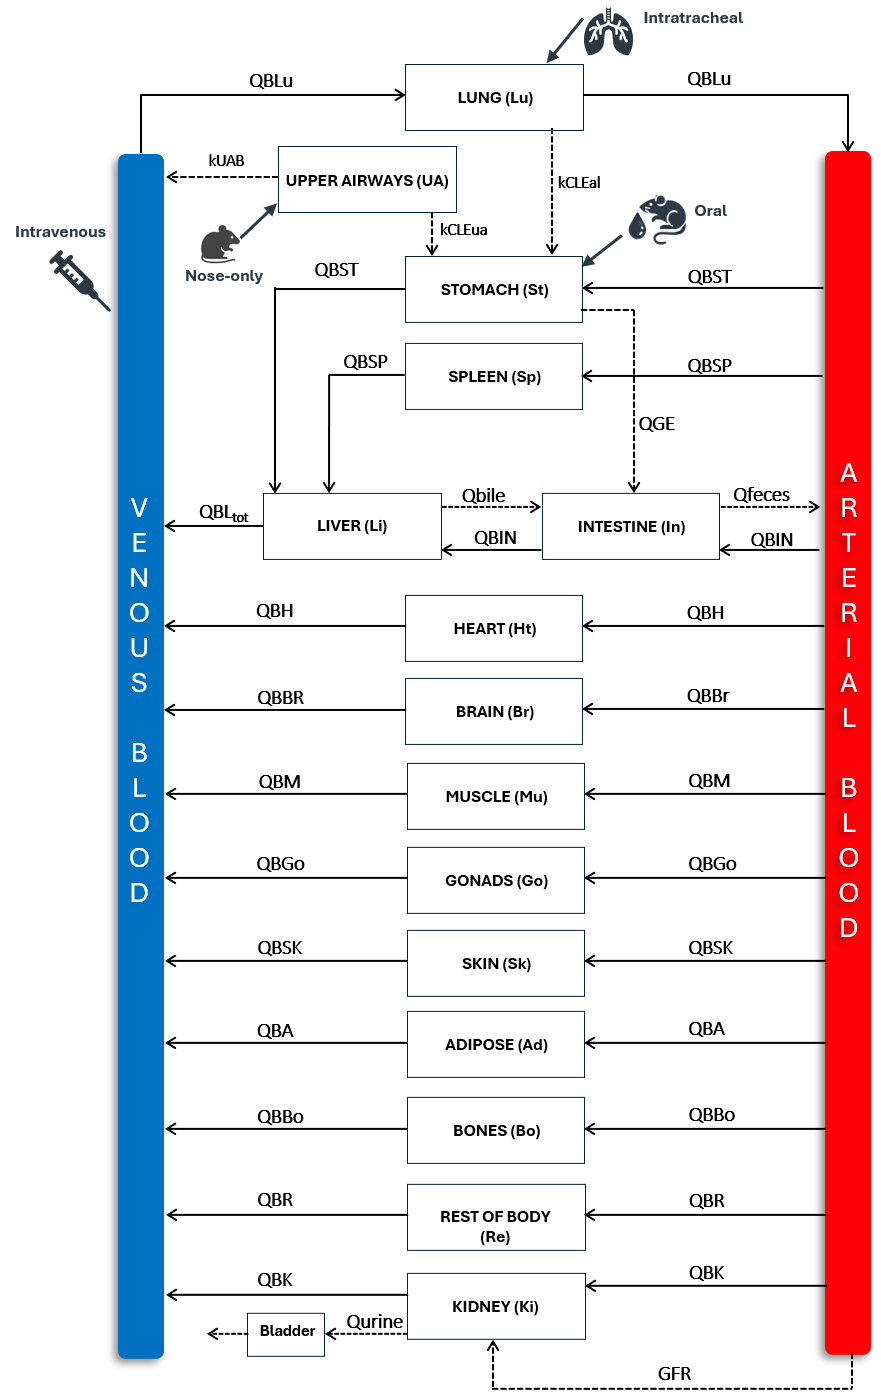
\includegraphics[width=0.75\textwidth]{Figures/whole_body_PBK.png}
    \caption{Schematic representation of the full-body PFOA PBK model in rats. Two compartments were used to represent the blood pool, namely venous blood (left, blue column) and arterial blood (right, red column). Fifteen compartments are vertically aligned, representing various organs/tissues (kidney, liver, stomach, intestine, lung, spleen, heart, brain, muscle, adipose, gonads, skin, bones, and rest of body). Solid arrows signify blood  flow, while dashed arrows signify flow of other fluids, e.g. bile.}
    \label{fig:whole_body_PBK}
\end{figure}

\subsubsection{Distribution}
Upon entering the systemic circulation, PFOA is distributed to various organs and tissues. Distribution to the lymph is unlikely due to the compound's physicochemical properties, particularly its anionic form under physiological conditions. This form increases its water solubility and reduces its tendency to partition into lipids \citep{post_2012}. The distribution of PFOA is governed primarily by two mechanisms: passive diffusion and active transport. 

Most compartments are subdivided into three subcompartments: the capillary blood, the interstitial fluid, and the intracellular compartment (Figure \ref{fig:PFOA_generic_compartment}). From the central blood pool, PFOA reaches the capillary blood of a tissue. It then permeates the endothelial barrier via transcellular diffusion and diffusion through gaps of the capillary endothelium. After passing through the endothelium, PFOA enters the interstitial fluid and, by passive diffusion, can subsequently enter the cells. In addition to these general compartments, there are tissue-specific spaces, such as the lumen in the stomach and intestine, and the epithelial lining fluid (ELF) in the lungs.


\begin{figure}[H]
    \centering
    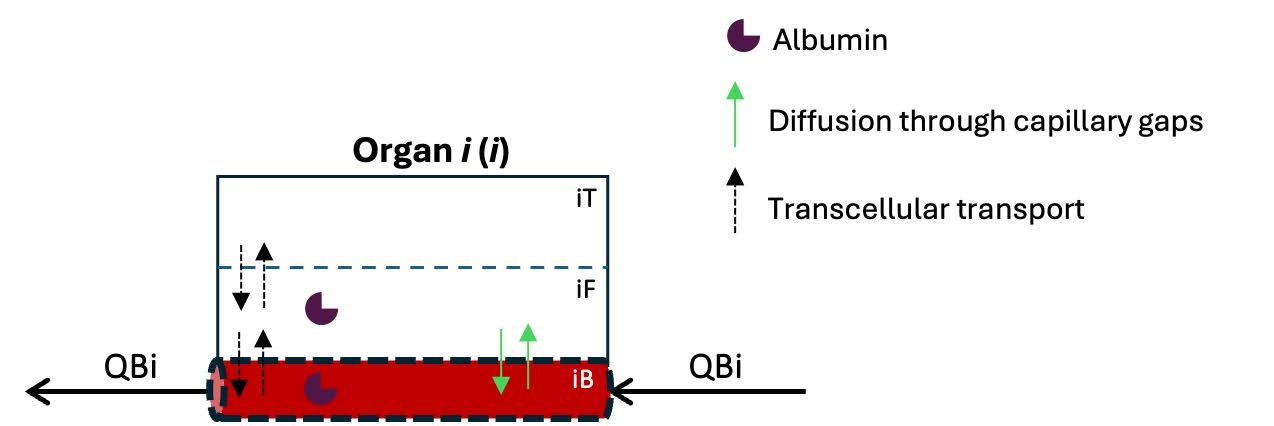
\includegraphics[width=1.0\textwidth]{Figures/generic_compartment.jpg}
    \caption{ Schematic representation of a generic organ compartment in the PFOA PBK model. Three  subcompartments were used to represent the regional capillary blood (iB), interstitial fluid (iF) and intracellular space (iT). Albumin (purple symbol) is assumed to be present in both the blood and interstitial fluid subcompartments. Green arrows indicate transport through capillary gaps, while black dashed arrows represent transcellular transport. Solid black arrows denote blood flow into and out of the organ compartment (QBi).}
    \label{fig:PFOA_generic_compartment}
\end{figure}



Active transport mediated by transporter proteins is considered in tissues where literature evidence supports its involvement \citep{niu_2023}. PFOA serves as a substrate for renal transporters expressed in rat kidneys, which facilitate both renal excretion and reabsorption. Most of the relevant transporters belong to the organic anion transporter (Oat) and organic anion transporting polypeptide (Oatp) families \citep{nakagawa_2008,weaver_2010, niu_2023}. Specifically, active secretion transporters Oat1 and Oat3 facilitate the movement of PFOA from the kidney's interstitial fluid to the intracellular compartment \citep{weaver_2010}. The reabsorption of PFOA from the proximal convoluted tubule back into the kidney proximal tubule cells is mediated by Oatp1a1 and the uric acid transporter (Urat) \citep{weaver_2010,zhang_2021, lin_2023}. In the liver, active transport also plays a role in the translocation of PFOA from the interstitial fluid to the intracellular compartment, with Oatp1a1 and Oatp2b1 functioning as uptake transporters in liver cells \citep{lin_2023}. Additionally, the sodium/taurocholate co-transporting polypeptide (Ntcp) transporter, expressed on the basolateral membranes of hepatocytes, contributes to PFOA uptake \citep{ruggiero_2021, zhao_2017}. Oatp2b1 is similarly expressed in the intestinal lumen, where it facilitates the apical uptake of PFOA from the lumen into intestinal cells \citep{zhao_2017, lin_2023}. Lastly, active transport is also considered in the lungs, as Oatp family transporters are expressed in lung tissue and facilitate PFOA uptake   \citep{kullakUblick_1995, ladumor_2022}.



Available literature indicates that albumin is the primary protein to which PFOA binds. The fraction of PFOA bound to plasma proteins has been found to account for over $90\%$ of the total PFOA following oral administration in rats \citep{han_2003}. The model considers the compartmental translocation of only the free fraction of PFOA, and thus, due to high protein binding, only a small portion remains free and available for transport across membrane barriers. Albumin is assumed to be present in both the capillary blood and interstitial fluid of all compartments, as well as in the ELF. Albumin is not assumed to be present in intracellular compartments, as it typically re-enters the bloodstream via the lymphatic system after crossing into the interstitial fluid \citep{moman_2022}. Therefore, while albumin is present in the fluids surrounding tissues, it is not stored or concentrated within the tissues. In addition to albumin, PFOA has been shown to bind to two specific intracellular proteins: $\alpha 2 u$-globulin (A2U) in kidney tissue, and liver fatty acid-binding protein (L-FABP) in both kidney and liver tissues. A2U  is a sex-specific protein located in the cytosol of rat kidneys, reported only in male subjects \citep{stonard_1986}. This sex difference was accounted for in the model, with the protein being considered only in male kidney tissue. The binding affinity of PFOA to L-FABP is a key factor in the potential bioaccumulation of PFAS in liver and kidney tissues. For several PFAS compounds, including PFOA, perfluorooctanesulfonic acid (PFOS), and related perfluorooctanesulfonamide-based fluorochemicals (PFOSAs), significant binding to L-FABP has been reported, which is attributed to their structural similarity to its natural substrate, fatty acids \citep{zhao_2023}. PFOA binding to L-FABP is accounted for in the model in both kidney and liver intracellular spaces. 

\subsubsection{Excretion}

The literature suggests that PFOA does not undergo metabolism \citep{atsdr_2021}, so its elimination primarily occurs via urine through glomerular filtration (GFR) in the kidneys and excretion via feces. After filtration, PFOA can either be directly cleared into the urine or undergo reabsorption, being transported back into the bloodstream \citep{efsa_2018}. Oat and Oatp kidney transporters are expressed in specific regions of the urinary tubule \citep{zhang_2021}, with reabsorption being more active in males. In female rats, elimination is predominantly governed by GFR \citep{loccisano_2012, worley_2015}. The fecal elimination pathway begins with the excretion of PFOA from the liver via bile. The chemical then reaches the small intestine, from where it can either be eliminated through feces or reabsorbed back into the intestinal tissue. Studies in rats have shown that the contribution of biliary excretion of PFOA is low due to the extensive reabsorption that occurs in the intestines \citep{atsdr_2015}.  

Given the significance of renal clearance in the observed PFOA dynamics, we chose to model the kidney with greater structural detail to gain a mechanistic understanding of the filtration and reabsorption processes. The kidney is thus divided into 11 subcompartments representing key tissue segments, including the proximal tubule cells (PTCs), cells of the loop of Henle (LHCs), consisting of the thin descending limb as well as the thin  and thick ascending limbs, the distal convoluted tubule cells (DTCs), the collecting duct cells (CDCs), and their respective luminal subcompartments. An additional subcompartment representing unspecified kidney cells is also included. These various cell types are connected to the interstitial fluid, which is modeled as a well-mixed, continuous, and uniform compartment in contact with all kidney cell types and the kidney capillary blood. The kidney compartment structure is illustrated in Figure \ref{fig:PFOA_kidney}. This higher resolution allows for modelling the reduction in urine flow along the renal tubule and also enables including distinct transporter expressions across different cell types. The glomerular filtrate enters the proximal tubule with a flow rate equal to the GFR, which gradually decreases along the tubule. PFOA leaving the collecting duct enters the bladder, from where it is finally excreted via urine. Regarding reabsorption, transporters Oatp1a1 and Urat are only considered in the proximal tubule cell subcompartment, as they are not expected to be significantly expressed in cells of other tubule regions \citep{zhang_2021}. Therefore, only passive diffusion is accounted for in the remaining renal tubule cells to describe the exchange between the filtrate lumen and tissue cells.


\begin{figure}[H]
    \centering
    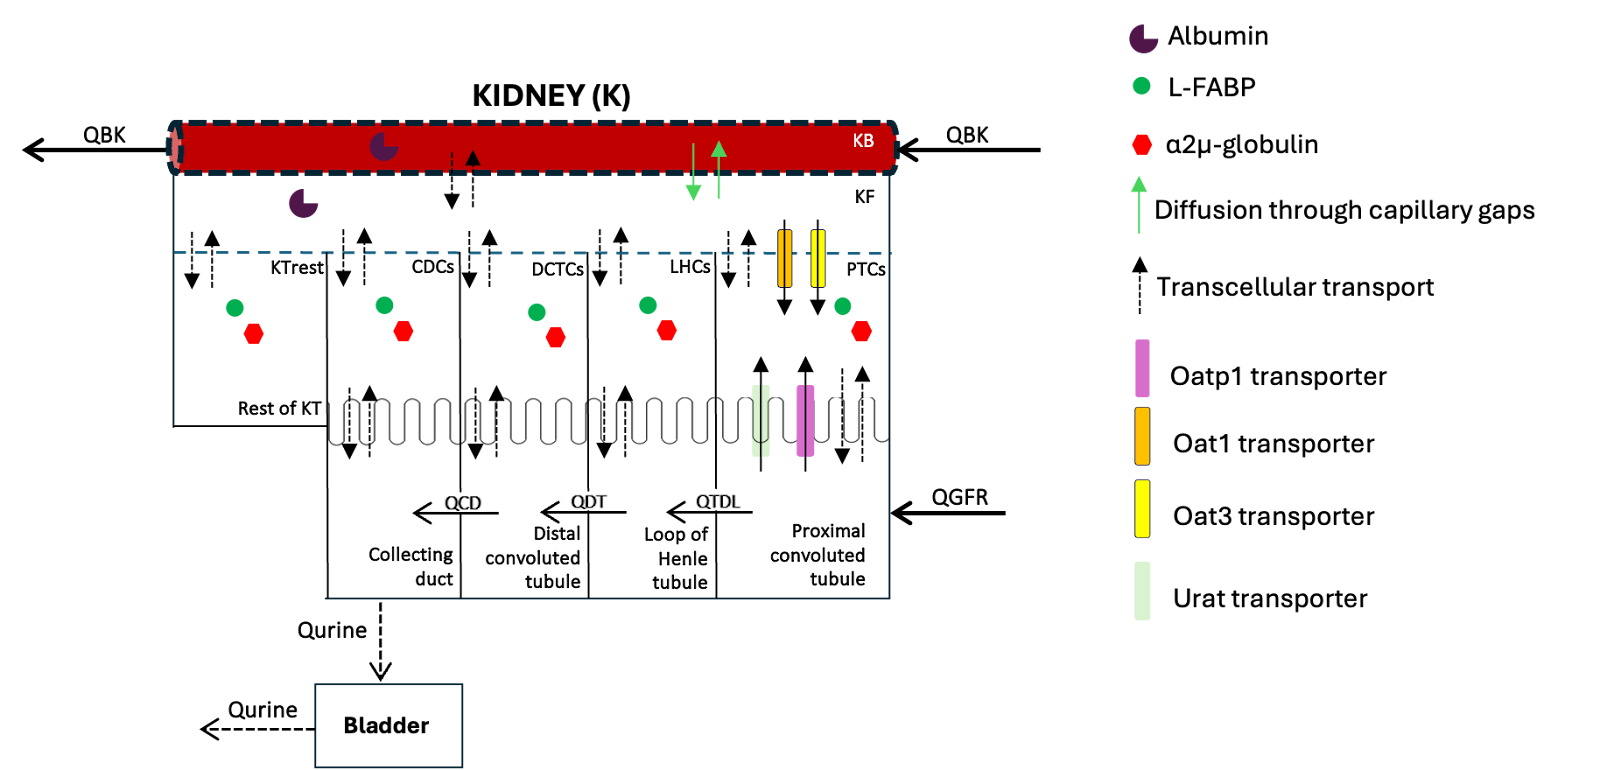
\includegraphics[width=1.0\textwidth]{Figures/kidney_struture.png}
    \caption{Schematic representation of the kidney structure in the PBK model in rats.}
    \label{fig:PFOA_kidney}
\end{figure}

Apart from the kidneys, other systems with structural intricacies are the lungs and the liver. Figure \ref{fig:PFOA_portal_organs} presents a schematic representation of the lungs and liver, along with the portal organs included in the model. 


\begin{figure}[H]
    \centering
    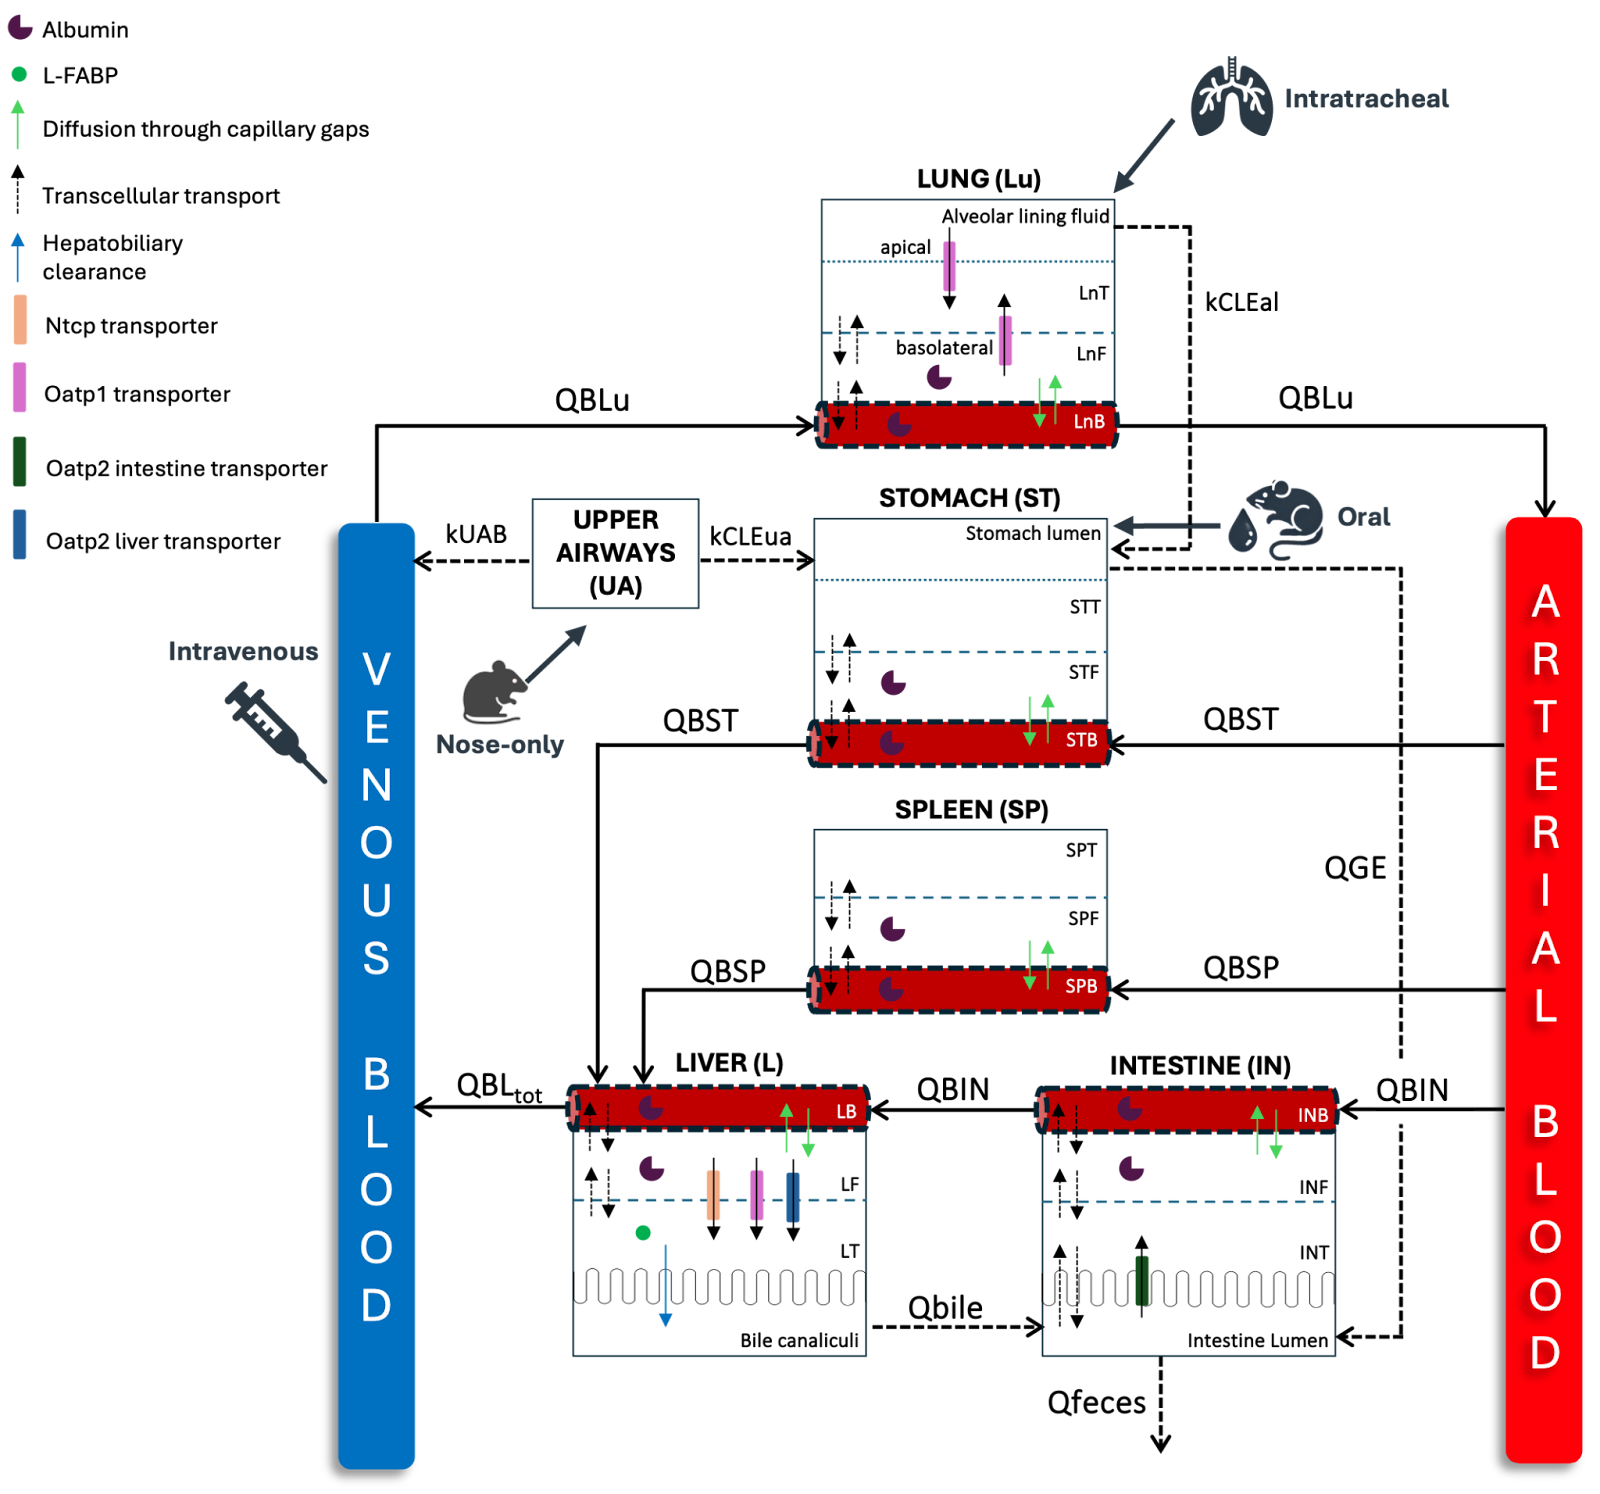
\includegraphics[width=1.0\textwidth]{Figures/GUT_system.png}
    \caption{Schematic representation of the lungs, liver, and portal organs compartmentalisation in the PBK model.}
    \label{fig:PFOA_portal_organs}
\end{figure}


\subsubsection{Mass Balance Equations}
Mass balance equations were used to model the distribution of PFOA within the organ compartments and subcompartments of each tissue. Each compartment is represented by ordinary differential equations (ODEs) that describe the change of free PFOA mass in all subcompartments, taking into account PFOA-protein interactions and exchanges between compartments. The generic ODE system for the capillary blood of organ $i$ is described by the following equations:

\begin{align}
\begin{aligned}
\frac{dM_{i,B}^f}{dt} &= Q_i \cdot C_{Art}^f 
- Q_i \cdot C_{i,B}^f \\
& \quad - (P_{trans}\cdot  (1-f_{i,gap}) + P_{i,para} \cdot f_{i,gap})  \cdot A_{i,B-IF} \cdot (C_{i,B}^f - C_{i,IF}^f) \\
& \quad + k_{off,alb} \cdot C_{i,B}^b \cdot V_{i,B} 
- k_{on,alb} \cdot C_{alb,i,B}^f \cdot C_{i,B}^f \cdot V_{i,B}
\end{aligned}
\label{eq:PFOA_blood_ODE_free_main}
\end{align}


The on- and off-rate binding constants are related to the association constant as:

\begin{align}
\begin{aligned}
K_a &= \frac{k_{on}}{k_{off}}
\end{aligned}
\label{eq:PFOA_association_constant_main}
\end{align}

The generic ODE system for the interstitial space of compartment $i$ is given by:

\begin{align}
\begin{aligned}
\frac{dM_{i,IF}^f}{dt} &= (P_{trans}\cdot  (1-f_{i,gap}) + P_{i,para} \cdot f_{i,gap}) \cdot A_{i,B-IF} \cdot (C_{i,B}^f - C_{i,IF}^f) \\ 
& \quad -  P_{cell} \cdot A_{i,IF-T} \cdot (C_{i,IF}^f - C_{i,T}^f) \\
& \quad + k_{off,alb} \cdot C_{i,IF}^b \cdot V_{i,IF} \\
& \quad - k_{on,alb} \cdot C_{alb,i,IF}^f \cdot C_{i,IF}^f \cdot V_{i,IF} \\
&  \quad - \sum_j \frac{V_{max,j} \cdot C_{i,IF}}{K_{m,j}+ C_{i,IF}}
\end{aligned}
\label{eq:PFOA_interstitial_ODE_free_main}
\end{align}


Finally, the generic ODE for the intracellular space of compartment $i$ is given by:

\begin{align}
\begin{aligned}
\frac{dM_{i,T}^f}{dt} &=  P_{cell} \cdot A_{i,IF-T} \cdot (C_{i,IF}^f - C_{i,T}^f) \\
&  \quad + \sum_j \frac{V_{max,j} \cdot C_{i,IF}}{K_{m,j}+ C_{i,IF}}  \\
+ \sum_p &  \big(k_{off,p} \cdot C_{i,T}^b \cdot V_{i,T} - k_{on,p} \cdot C_{p,i,T}^f \cdot C_{i,T}^f \cdot V_{i,T} \big)\\
\end{aligned}
\label{eq:PFOA_tissue_ODE_main}
\end{align}

where $M$, $C$, and $V$ denote mass, concentration, and volume, respectively; subscripts $B$, $IF$, and $T$ refer to capillary blood, interstitial fluid, and intracellular space (tissue), respectively; and superscripts $f$ and $b$ denote the fraction of free PFOA and the fraction bound to protein, respectively. For example, $M_{i,IF}^f$ represents the mass of free PFOA in the interstitial fluid of compartment $i$, while $M_{i,IF}^b$ represents the mass of albumin-bound PFOA in the same compartment. $C_{alb,i,B}^f$ and $C_{alb,i,IF}^f$ are the concentrations of unoccupied albumin binding sites in capillary blood and interstitial fluid, respectively. $Q_i$ is the blood flow to compartment $i$, and $A_{i,B-IF}$ and $A_{i,IF-T}$ represent the surface areas between capillary blood and interstitial fluid, and between interstitial fluid and tissue. $P_{trans}$, $P_{para}$ and $P_{cell}$ are the permeability coefficients for transcellular transport, paracellular transport and cellular uptake respectively, while $f_{i,gap}$ is the fraction of the endothelial surface area covered by gaps. $k_{on,alb}$ and $k_{off,alb}$ are the on- and off-rate constants for albumin binding, and $K_a$ is the albumin association constant. $V_{max,j}$ and $K_{M,j}$ denote the maximum transport velocity and the affinity constant of transporter $j$. The transporters apply only to the case of the lung, liver and kidney compartments. Transporters also mediate the uptake of PFOA from ELF to lung tissue, from intestine lumen to intestine tissue and from proximal tubule lumen to proximal tubule cells. Protein binding in the intracellular space is only considered for the kidney and liver compartments. The analytical mass balance equations for all compartments are provided in Supplemental Material (SM) section \ref{Appendix:PFOA_mass_balance}.

\subsection{Model Parameterisation}
\subsubsection{\textit{In vitro} data}
A middle-out approach employing \textit{in vitro} and \textit{in vivo} data was followed for parameterising the PBK model. The apparent permeability from a monolayer assay using the MDCK-LE cell line was used to represent PFOA membrane permeability \citep{rue_2024}. Half of the monolayer permeability was used to represent single membrane permeation, which occurs during cellular uptake. Based on the findings of \citet{ryu_2024}, the influence of pH on PFOA permeability was minimal, probably due to the pKa of PFOA reported to range from 0.5 to 3.8 \citep{burns_2008}. Consequently, the same permeability value was used for endothelium permeation, intestinal absorption, and cellular uptake, including uptake by tubular cells. The \textit{in vitro} transporter parameters used for developing the model are presented in Table \ref{Table:transporter_Km_Vmax}. The scaling process of the maximum transport velocity is presented in SM section \ref{Appendix:toxicokinetics}. Binding affinities to different proteins, including albumin, A2U and L-FABP were either derived from the literature or estimated through parameter calibration.

\begin{table}[H]
\centering
\caption{Transporter $K_m$ and $V_{max}$ values from \textit{in vitro} assays used for model development.}
\label{Table:transporter_Km_Vmax}
\resizebox{\textwidth}{!}{
\begin{tabular}{cccrrl}
\toprule
\textbf{Transporter} & \textbf{Organ} & \textbf{Transport process} & \shortstack{$\boldsymbol{K_m}$ \\ ($\mu mol/L$)} & \shortstack{$\boldsymbol{V_{max}}$ \\ ($nmol/mg$\textsubscript{\textit{prot}}$/min$)}
 & \textbf{Reference} \\
\midrule
Oat3 & kidney & KF to KT & 65.7 & 3.8 & \citep{weaver_2010}\\
Oat1 & kidney & KF to KT & 43.2 & 2.6 & \citep{weaver_2010} \\
Urat & kidney & PT to KT & 820.0 & 1.5 & \citep{lin_2023} \\
Oatp1a1 & kidney & PT to KT & 126.4 & 9.3 &\citep{weaver_2010} \\
Oatp1a1 & liver & LF to LT & 126.4 & 9.3 & same as kidney \\
Oatp2b1 & liver & LF to LT & 148.7 & 1.5 & \citep{lin_2023} \\
Ntcp & liver & LF to LT & 20.0 & 3.0 & \citep{ruggiero_2021}\\
Oatp2b1 & intestine & INL to INT & 8.3 & 0.5 & \citep{kimura_2017} \\

Oatp & lung & LuF to LuT & 126.4 & 9.3 & same as kidney\\
\bottomrule
\end{tabular}
}

\raggedright
\footnotesize
\vspace{0.5em}
\raggedright
\scriptsize
BC: bile canaliculi; ELF: epithelial lining fluid; INL: intestinal lumen; INT: intestinal tissue; KF: kidney interstitial fluid; KT: kidney tissue; LF: liver interstitial fluid; LT: liver tissue; LuF: lung interstitial fluid; LuT: lung tissue; Ntcp: sodium/taurocholate co-transporting polypeptide; Oat1: organic anion transporter 1; Oat3: organic anion transporter 3; Oatp1a1: organic anion transporting polypeptide 1A1; Oatp2b1: organic anion transporting polypeptide 2B1; Urat: uric acid transporter.
\end{table}


\subsubsection{Animal Biodistribution Data}
Animal data from six different studies, presented in Table \ref{Table:animal_studies}, were utilized for model development. These studies provided different biodistribution data covering a wide range of administration routes, doses and tissues for both male and female rats, allowing investigation of possible dose effects and/or sex differences. Specifically, the model was developed using data covering a dose range from 0.041 to 320 $mg/kg$ of body weight, with both single and repeated dosing schemes, enabling modelling of  both low and high doses as well as PFOA accumulation after repeated exposure. Concentration-time data points were extracted from published plots using plot digitisation \citep{webPlotDigitizer}. For most tissues, only single concentration-time pairs were available, whereas more comprehensive time series data were limited to  blood, liver, kidney, brain, urine and feces. 

\begin{table}[H]
\centering
\caption{Animal studies used for model development.}
\label{Table:animal_studies}
\resizebox{\textwidth}{!}{
\begin{tabular}{lrlcl}
\toprule
\textbf{Exposure Route} & \textbf{\shortstack{Dose \\ (mg/kg BW)}} & \textbf{Tissue} & \textbf{Sex} & \textbf{Reference} \\
\midrule
IV/oral & 6, 12, 40, 48, 80, 320 & plasma, liver, kidney, brain & M/F & \citep{dzierlenga_2020} \\
\multirow[t]{2}{*}{oral/} & \multirow[t]{2}{*}{0.364 (oral)} & plasma, ELF, lung, & \multirow[t]{2}{*}{M} & \multirow[t]{2}{*}{\citep{gustafsson_2022}} \\
intratracheal inhalation & 0.164 (inhalation) & liver, kidney & & \\
nose-only inhalation & 0.27, 0.96, 2 & serum & M/F & \citep{hinderliter_2006} \\
oral & 1, 5, 25 & urine, feces & M/F & \citep{kemper_2003} \\
IV/oral & 1 & blood, liver, kidney, lung, spleen, heart & M/F & \citep{kim_2016} \\
\multirow[t]{3}{*}{IV} & \multirow[t]{3}{*}{0.041, 16.56} & blood, liver, kidney, carcass\textsuperscript{1}, & \multirow[t]{3}{*}{M} & \multirow[t]{3}{*}{\citep{kudo_2007}} \\
& & lung, spleen, heart, brain, & & \\
& & gonads, stomach, intestine & & \\
\bottomrule
\end{tabular}
}

\raggedright
\footnotesize
\vspace{0.5em}
\raggedright
\scriptsize
BW: body weight; ELF: epithelial lining fluid; F: female;  IV: intravenous; M: male \\
\textsuperscript{1} Carcass was assumed to correspond to the sum of the muscle, adipose, bones, skin, and RoB model compartments.
\end{table}



\subsubsection{Physiological data}
Physiological parameters for rats were sourced from several literature sources. These parameters include the total albumin concentration in the capillary blood and interstitial fluid, the regional blood flows, capillary blood, interstitial fluid and intracellular space volumes, as well as the capillary and interstitial – intracellular surface areas of each tissue. Physiological parameter values employed in modelling are summarized in Table \ref{Table:PFOA_Parameters}. 

\subsection{Parameter calibration}
To address parameters for which \textit{in vitro} parameterization was either not feasible or highly uncertain, calibration was conducted using the concentration-time profiles of female or male rats following single or repeated exposure through the IV, inhalation or oral routes (Table \ref{Table:animal_studies}). In model simulations, the reported average rat body weight of each study was used. For studies that did not specify the body weight, a default value equal to 0.25 kg was applied. For each exposure scenario, the total organ concentration was calculated by summing the mass of the organ subcompartments and dividing by the total organ volume. For each sample, the simulated total organ concentration was then compared to the corresponding reported concentration  using the absolute average fold error ($AAFE$) metric: 

\begin{equation}
AAFE = 10^{\frac{1}{n}\sum  \log_{10} \left( \frac{y_{predicted}}{y_{observed}} \right)  }
\end{equation}

\noindent
where $y_{predicted}$ is the predicted concentration, $y_{observed}$ is the observed concentration, and $n$ is the number of observations in the dataset. Parameters were calibrated through optimisation, aiming to minimise the average $AAFE$ across all datasets.


Similar to previous efforts, calibrated relative activity factors (RAFs) were used to account for differences between the maximum transport velocity extrapolated to \textit{in vivo} from \textit{in vitro} experiments and the actual  \textit{in vivo} transport \citep{worley_2015}. These differences can be attributed mainly to differences in the expression of transporters between the  \textit{in vitro} and  \textit{in vivo} systems. Therefore, RAFs of membrane transporters mediating PFOA uptake or efflux in the kidneys (Oatp1a1, Oat3, Oat1, Urat), liver (Oatp1a1, Oatp2b1, Ntcp), intestine (Oatp2b1), and lung were estimated by fitting the model on the available  \textit{in vivo} data. To reduce the number of estimated parameters, apical lung transporter activity was assumed negligible, as no specific literature evidence on the localisation of lung transporters was available. Furthermore, a single RAF value was assumed for transporters that share the same transport direction within the same organ, due to parameter identifiability restrictions.

To describe both transcellular and paracellular transport, the fraction of endothelial gaps in each organ was obtained from the literature. Rather than applying a uniform paracellular permeability coefficient across all organs, the specific capillary type of each organ was taken into account. In particular, the upper pore size limit reported by \citet{sarin_2010} enabled the physiological distinction between continuous, fenestrated, and sinusoidal capillaries. Based on pore size, the diffusion coefficient of PFOA in water, steric hindrance, hydrodynamic drag reductions in diffusion \citep{renkin_1954}, and the average diffusion distance, an upper permeability threshold for diffusion through pores was estimated. However, additional unaccounted factors, such as the glycocalyx, could further reduce permeability. For instance, \citet{Gao_2010} demonstrated that the free diffusion coefficient of a fluorescent dye in solution was approximately three orders of magnitude higher than within the glycocalyx. Accordingly, an additional permeability reduction factor was introduced and applied across all organs. Further details are provided in the Supplemental Material.

 A wide range of parameter values was reported in the literature for the equilibrium association constant of albumin. Consequently, due to high uncertainty, this parameter was also fitted to the data. Hepatobiliary and fecal clearances were also calibrated using the \textit{in vivo} data. Finally, the parameters of the respiratory system, including the absorption rate of PFOA from the nasal cavity to the blood stream, as well as the desorption rate from dust to the epithelial lining fluid, were also calibrated, bringing the total number of estimated model parameters to 11, and another 4 parameters that were specific to only one scenario.




\subsection{Model  Validation}
To evaluate the robustness of the model, independent datasets beyond those used for calibration were employed to assess its predictive performance across various scenarios. The calibrated model was used to simulate concentration–time profiles under defined exposure conditions, and the results were compared with corresponding experimental observations. Predictions for single and repeated exposures at different doses and routes in both male and female rats were evaluated. The experimental data used for validation are summarised in Table \ref{Table:animal_validation}.

\begin{table}[H]
\centering
\caption{Animal studies used for model validation.}
\label{Table:animal_validation}
\resizebox{\textwidth}{!}{
\begin{tabular}{lrlcll}
\toprule
\textbf{Exposure Route} & \textbf{\shortstack{Dose \\ (mg/kg BW)}} & \textbf{Tissue} & \textbf{Sex} & \textbf{Reference} \\
\midrule
\multirow[t]{3}{*}{oral} & \multirow[t]{3}{*}{5, 20 (per day)} & liver, kidney, lung, & \multirow[t]{2}{*}{M} & \multirow[t]{3}{*}{\citep{cui_2010}} \\
& & spleen, heart, brain, gonads & & \\
& & urine, feces & & \\
nose-only inhalation & 0.27, 0.96, 2 (per day) & plasma & M/F & \citep{hinderliter_2006} \\
IV/oral & 1, 5, 25 & serum & M/F & \citep{kemper_2003} \textsuperscript{1} \\
oral & 0.047 (per 12 h) & urine, feces, liver, skin, kidney & F & \citep{lupton_2021} \\
\midrule
\end{tabular}
}

\raggedright
\footnotesize
\vspace{0.5em}
\raggedright
\scriptsize
F: female; IV: intravenous; M: male\\
\textsuperscript{1} The data from \citet{kemper_2003} were retrieved from the compilations presented in \citet{loccisano_2012} and \citet{worley_2015}. 
\\
\end{table}


\subsection{Sensitivity analysis}
Local sensitivity analysis was performed for a set of model parameters considered important to identify the most influential parameters in each compartment. A $50\%$ perturbation was applied to each parameter, and sensitivity was assessed by comparing changes in the AUC for each compartment relative to the baseline values. The sensitivity index of parameter $j$ on compartment $i$ was calculated by the following formula:

\begin{equation}
SI_{i,j} = 100\% \times \left( \frac{\Delta AUC_i / AUC_i}{\Delta \theta_j / \theta_j} \right)
\end{equation}

\noindent
where $AUC_i$ represents the area under the curve of the response variable $i$, $\Delta AUC_i$ denotes the change in the AUC due to a 50\% increase in the parameter value, $\theta_j$ is the initial value of parameter $j$, and $\Delta \theta_j$ corresponds to 50\% of the original value of parameter $j$.





\subsection{Software}
The PBK model was coded in the R programming language v.4.0.4 \citep{rcore_2021}. The ODE system was solved using the lsodes algorithm of deSolve package \citep{soetaert_2010}. Parameter calibration was implemented using the NEWUOA method \citep{powell_2006} through the nloptr package \citep{johnson_2025}. The R code of the model can be found in: \url{https://github.com/ntua-unit-of-control-and-informatics/multi-route-pbk-pfoa} 


\section{Results}

Model calibration allowed the estimation of a total of 16 model and scenario-related parameters.  Prior to this final parameter list, various combinations of sex-dependent chemical-specific parameters were tested. For most parameters, distinguishing between males and females did not significantly improve the model fit to the \textit{in vivo} data, and therefore, sex-invariant values were used for the sake of parsimony. However, for the RAF of the Oatp1a1  and Urat transporters in the kidney, using different parameter values for males and females notably enhanced the model fit. Importantly, incorporating sex-specificity for this parameter alone was sufficient for the model to accurately reproduce the observed differences in PFOA biodistribution between males and females. Finally, the potential influence of experiment duration, which can introduce growth dilution effects, was examined. Body weight was updated at each time point using reported growth rates of 5.9 g/day for males and 3.5 g/day for females \citep{ghasemi_2021}, with upper limits of 0.6 kg and 0.375 kg applied for male and female rats, respectively. This adjustment was intended to account for differences in experimental duration between sexes. However, the results indicated that growth dilution had little impact on the model outputs. To reduce computational complexity, body weight adjustment was therefore omitted from the final model.


The values of all chemical-specific and scenario-related parameters are presented in Table \ref{Table:parameters}. The RAF values for the liver transporters Oatp1a1/ Oatp2b1/ Ntcp, as well as for the lung Oatp transporters (assumed to be localised exclusively at the basolateral membrane), were found to be close to unity. This suggests that differences in specific transporter activity between the tested \textit{in vitro} and \textit{in vivo} systems are minimal for the particular transporter species. In contrast, the RAF of Oatp1a1 in the female kidney was markedly lower than unity and significantly lower than the corresponding male value, an observation that may be attributed hormonal regulation of transporter expression \citep{lu_1996, wood_2005}. The RAF values for Oat1/ Oat3 were unexpectedly high, likely reflecting optimisation attempts to reduce systemic PFOA levels. Finally, the intestinal transporter Oatp2b1 was essentially inactive, indicating that passive diffusion alone was sufficient to account for the observed \textit{in vivo} absorption.


Binding to proteins is key in describing the biodistribution patterns of PFOA. To reduce computational complexity and avoid identifiability problems, all off-rate constants were set to $10^{-2}$ 1/s, reflecting very fast binding in relation to PFOA distribution kinetics. Thus, almost instant binding was assumed, and the significance of using explicit binding dynamics lied on describing the binding site saturation at high doses, as illustrated in Figure \ref{fig:fu_plot}. The binding affinities of PFOA to A2U and L-FABP were obtained from published \textit{in vitro} experiments. For albumin, however, reported values vary widely, ranging from $6 \cdot 10^2$ \citep{macmanuspencer_2010} to $9 \cdot 10^6$ L/mol \citep{crisalli_2023}, reflecting differences in experimental methods and conditions. This variability made calibration against \textit{in vivo} data essential. The association constant for albumin was estimated to be approximately $2.4 \cdot 10^4$ L/mol. In contrast, attempts to apply literature-derived values were unsuccessful, even when using the fraction unbound of PFOA in rat plasma to back-calculate the constant. In that case, the resulting value was much higher ($5.6 \cdot 10^5$ L/mol), which led to excessive binding and an underprediction of clearance, particularly in female rats (Figure \ref{fig:protein_binding}).

Both intratracheal and nasal inhalation experiments were used to parameterise the respiratory system. To stabilise the estimation process, and given the near-complete bioavailability of PFOA, clearance terms from both the lower and upper respiratory tract to the stomach were fixed to zero. The study of \citet{gustafsson_2022}, which included desorption of PFOA from deposited dust, was represented using a fast and a slow desorption fraction, reflecting the formation of PFOA pools with different degrees of accessibility \citep{gustafsson_2022}. In addition, the fraction of rapidly desorbing dust was estimated, along with the proportion of PFOA in the ELF that remains after bronchoalveolar lavage (BAL).


Both intratracheal inhalation and nasal inhalation experiments were used to parameterise the respiratory system. To stabilise the estimation process and due to the near complete bioavailability of PFOA, the clearance terms from both the lower and upper respiratory systems to the stomach were set to zero. The experiment of \citet{gustafsson_2022}, which included desorption of PFOA from deposited dust, was modelled using a two desorption fractions, a slow and a fast one, reflecting the fact that the PFOA sorption process possibly creates PFOA pools of different accessibility \citep{gustafsson_2022}. The fraction of fast desorpting dust was also estimated, in addition to the fraction of PFOA in the ELF that is not recovered during brochoalveolar lavage (BAL).

\begin{table}[H]
\centering
\caption{Chemical-specific model parameters and scenario-related parameters.}
\label{Table:parameters}
\resizebox{\textwidth}{!}{
\begin{tabular}{clrcl}
\toprule
\textbf{Symbol} & \textbf{Definition} & \textbf{Value} & \textbf{Unit} & \textbf{Source} \\
\midrule
\multirow[t]{2}{*}{$RAF_{Oatp1a1/ Urat,Ki}$} & relative activity factor & $1.6\cdot 10^{1}$ (M) & \multirow[t]{2}{*}{-} & \multirow[t]{2}{*}{calibrated} \\
& of Oatp1a1 in kidneys & $4.0\cdot 10^{-3}$ (F) & & \\
\multirow[t]{2}{*}{$RAF_{Oat3/Oat1,Ki}$} & relative activity factor  & \multirow[t]{2}{*}{$9.8 \cdot 10^3$} & \multirow[t]{2}{*}{$-$} & \multirow[t]{2}{*}{calibrated} \\
& of Oat1 \& Oat3 in kidneys & & & \\
\multirow[t]{2}{*}{$RAF_{Oatp1a1/Oatp2b1/Ntcp,Li}$} & relative activity factor of Oatp1a1,  & \multirow[t]{2}{*}{$5.0 \cdot 10^{-1}$} & \multirow[t]{2}{*}{$-$} & \multirow[t]{2}{*}{calibrated} \\
& Oatp2b1 \& Urat in liver & & & \\
\multirow[t]{2}{*}{$RAF_{Oatp,Lu}$} & relative activity factor of Oatp & \multirow[t]{2}{*}{$4.2 \cdot 10^{-1}$} & \multirow[t]{2}{*}{$-$} & \multirow[t]{2}{*}{calibrated} \\
& in lung & & & \\
\multirow[t]{2}{*}{$RAF_{Oatp2b1, In}$} & relative activity factor of Oatp2b1 & \multirow[t]{2}{*}{$6.2\cdot 10^{-6}$} & \multirow[t]{2}{*}{$-$} & \multirow[t]{2}{*}{calibrated} \\
& in intestine & & & \\
\multirow[t]{2}{*}{$P_{app}$} & permeability coefficient used for parameterising $P_{cell}$ and $P_{trans}$  & \multirow[t]{2}{*}{$1.5 \cdot 10^{-6}$} & \multirow[t]{2}{*}{$cm/s$} & \multirow[t]{2}{*}{calibrated} \\
& permeability coefficients & & & \\
\multirow[t]{2}{*}{$f_{r}^ {\quad a}$} & reduction factor for $P_{para}$ & \multirow[t]{2}{*}{$3.7 \cdot 10^{-2}$} & \multirow[t]{2}{*}{$-$} & \multirow[t]{2}{*}{\citep{ryu_2024}} \\
&  & & & \\
$K_{a,alb}$ & albumin association constant & $ 2.4 \cdot 10^4$ & $L/mol$ & calibrated \\
$K_{a,fabp}$ & L-FABP association constant &  $1.2 \cdot 10^5$ & $L/mol$ & \citep{sheng_2018} \\
$K_{a,a2u}$ & A2U association constant & $ 1.0 \cdot 10^3$ & $L/mol$ & \citep{han_2004} \\
$k_{off,alb}$ & off-rate from albumin & $1.0 \cdot 10^{-2}$ & $1/s$ & assumed \\
$k_{off,fabp}$ & off-rate from L-FABP &  $1.0 \cdot 10^{-2}$ & $1/s$ & assumed \\
$k_{off,a2u}$ & off-rate from A2U & $1.0 \cdot 10^{-2}$ & $1/s$ & assumed \\
\multirow[t]{2}{*}{$CL_{biliary}$} & biliary clearance  & \multirow[t]{2}{*}{$2.0$} & \multirow[t]{2}{*}{$\mu L/min/million\ hepatocytes$} & \multirow[t]{2}{*}{calibrated} \\
& from liver to duodenum & & & \\
$CL_{feces}$ & clearance from IL to feces & $8.2 \cdot 10^{-5}$ & $L/h/BW^{-0.25}$ & calibrated \\
$k_{UAB}$ & absorption from UA to blood & $1.0 \cdot 10^{-1}$ & $L/h/m^2$ & calibrated \\
$CL_{ELF}$ & clearance from  ELF to SL & $0$ & $1/h$ & assumed \\
$CL_{UA}$ & clearance from UA to SL& $0$ & $1/h$ & assumed \\
$k_{desorption, fast}^{\quad a,b}$ & fast desorption rate from dust & $10.9$ & $1/h$ & calibrated \\
$k_{desorption, slow}^ {\quad a,b}$ & slow desorption rate from dust & $1.3 \cdot 10^{-2}$ & $1/h$ & calibrated \\
$f_{fast}^ {\quad a,b}$ & fraction of PFOA that undergoes fast desorption & $5.8 \cdot 10^{-1}$ & $-$ & calibrated \\
$f_{retained}^ {\quad a,b}$ & fraction of retained PFOA after BALF & $5.8 \cdot 10^{-1}$ & $-$ & calibrated \\
\bottomrule
\end{tabular}
}

\raggedright
\footnotesize
\vspace{0.5em}
\raggedright
\scriptsize
A2U: alpha 2u-globulin; ELF: epithelial lining fluid; F: female; IL: intestine lumen ; L-FABP: liver fatty-acid binding protein;  M: male; SL: stomach lumen; UA: upper airways
\newline
$^a$: check Supplemental Material for more details
$^b$: used only in the case study of \citet{gustafsson_2022}. For more details the user is referred to the Supplemental Material.
\end{table}

Model simulations were evaluated for their ability to reproduce both peak concentrations and the overall shape of the concentration–time profiles. Visual inspection was first used to compare predicted and observed values, ensuring that simulated trends were consistent with the experimental data. In parallel with this qualitative assessment, quantitative evaluation was performed using the $AAFE$ between predictions and observations. Across all calibration studies, the total $AAFE$ was 2.15. Table \ref{Table:sup_calibration_aafe} summarises the average $AAFE$ values for each study, reporting separate values by compartment type (excreta, serum, tissues), sex, and administration route. In most cases, the $AAFE$ was close to the threshold value of two, which has been proposed as an acceptable limit for model quality by \citet{who_2010}.

In most cases, the model demonstrated very good performance, accurately capturing the dynamics of PFOA in both female and male rats. Figure \ref{fig:serum_gof} shows the goodness-of-fit to the serum concentration–time profiles reported by \citet{dzierlenga_2020}, who investigated PFOA biodistribution in male and female rats across a wide range of doses administered by both intravenous and oral routes. Figure \ref{fig:excreta_gof} presents the fit to urine and feces mass–time data from male and female rats following oral administration at different dose levels \citep{kemper_2003}. Additional results are provided in Figures \ref{fig:experiment1}–\ref{fig:experiment15} in the Supplemental Material, illustrating model predictions against observed data from the studies of \citet{kudo_2007}, \citet{kim_2016}, \citet{gustafsson_2022}, and \citet{hinderliter_2006}.


\begin{figure}[H]
    \centering
    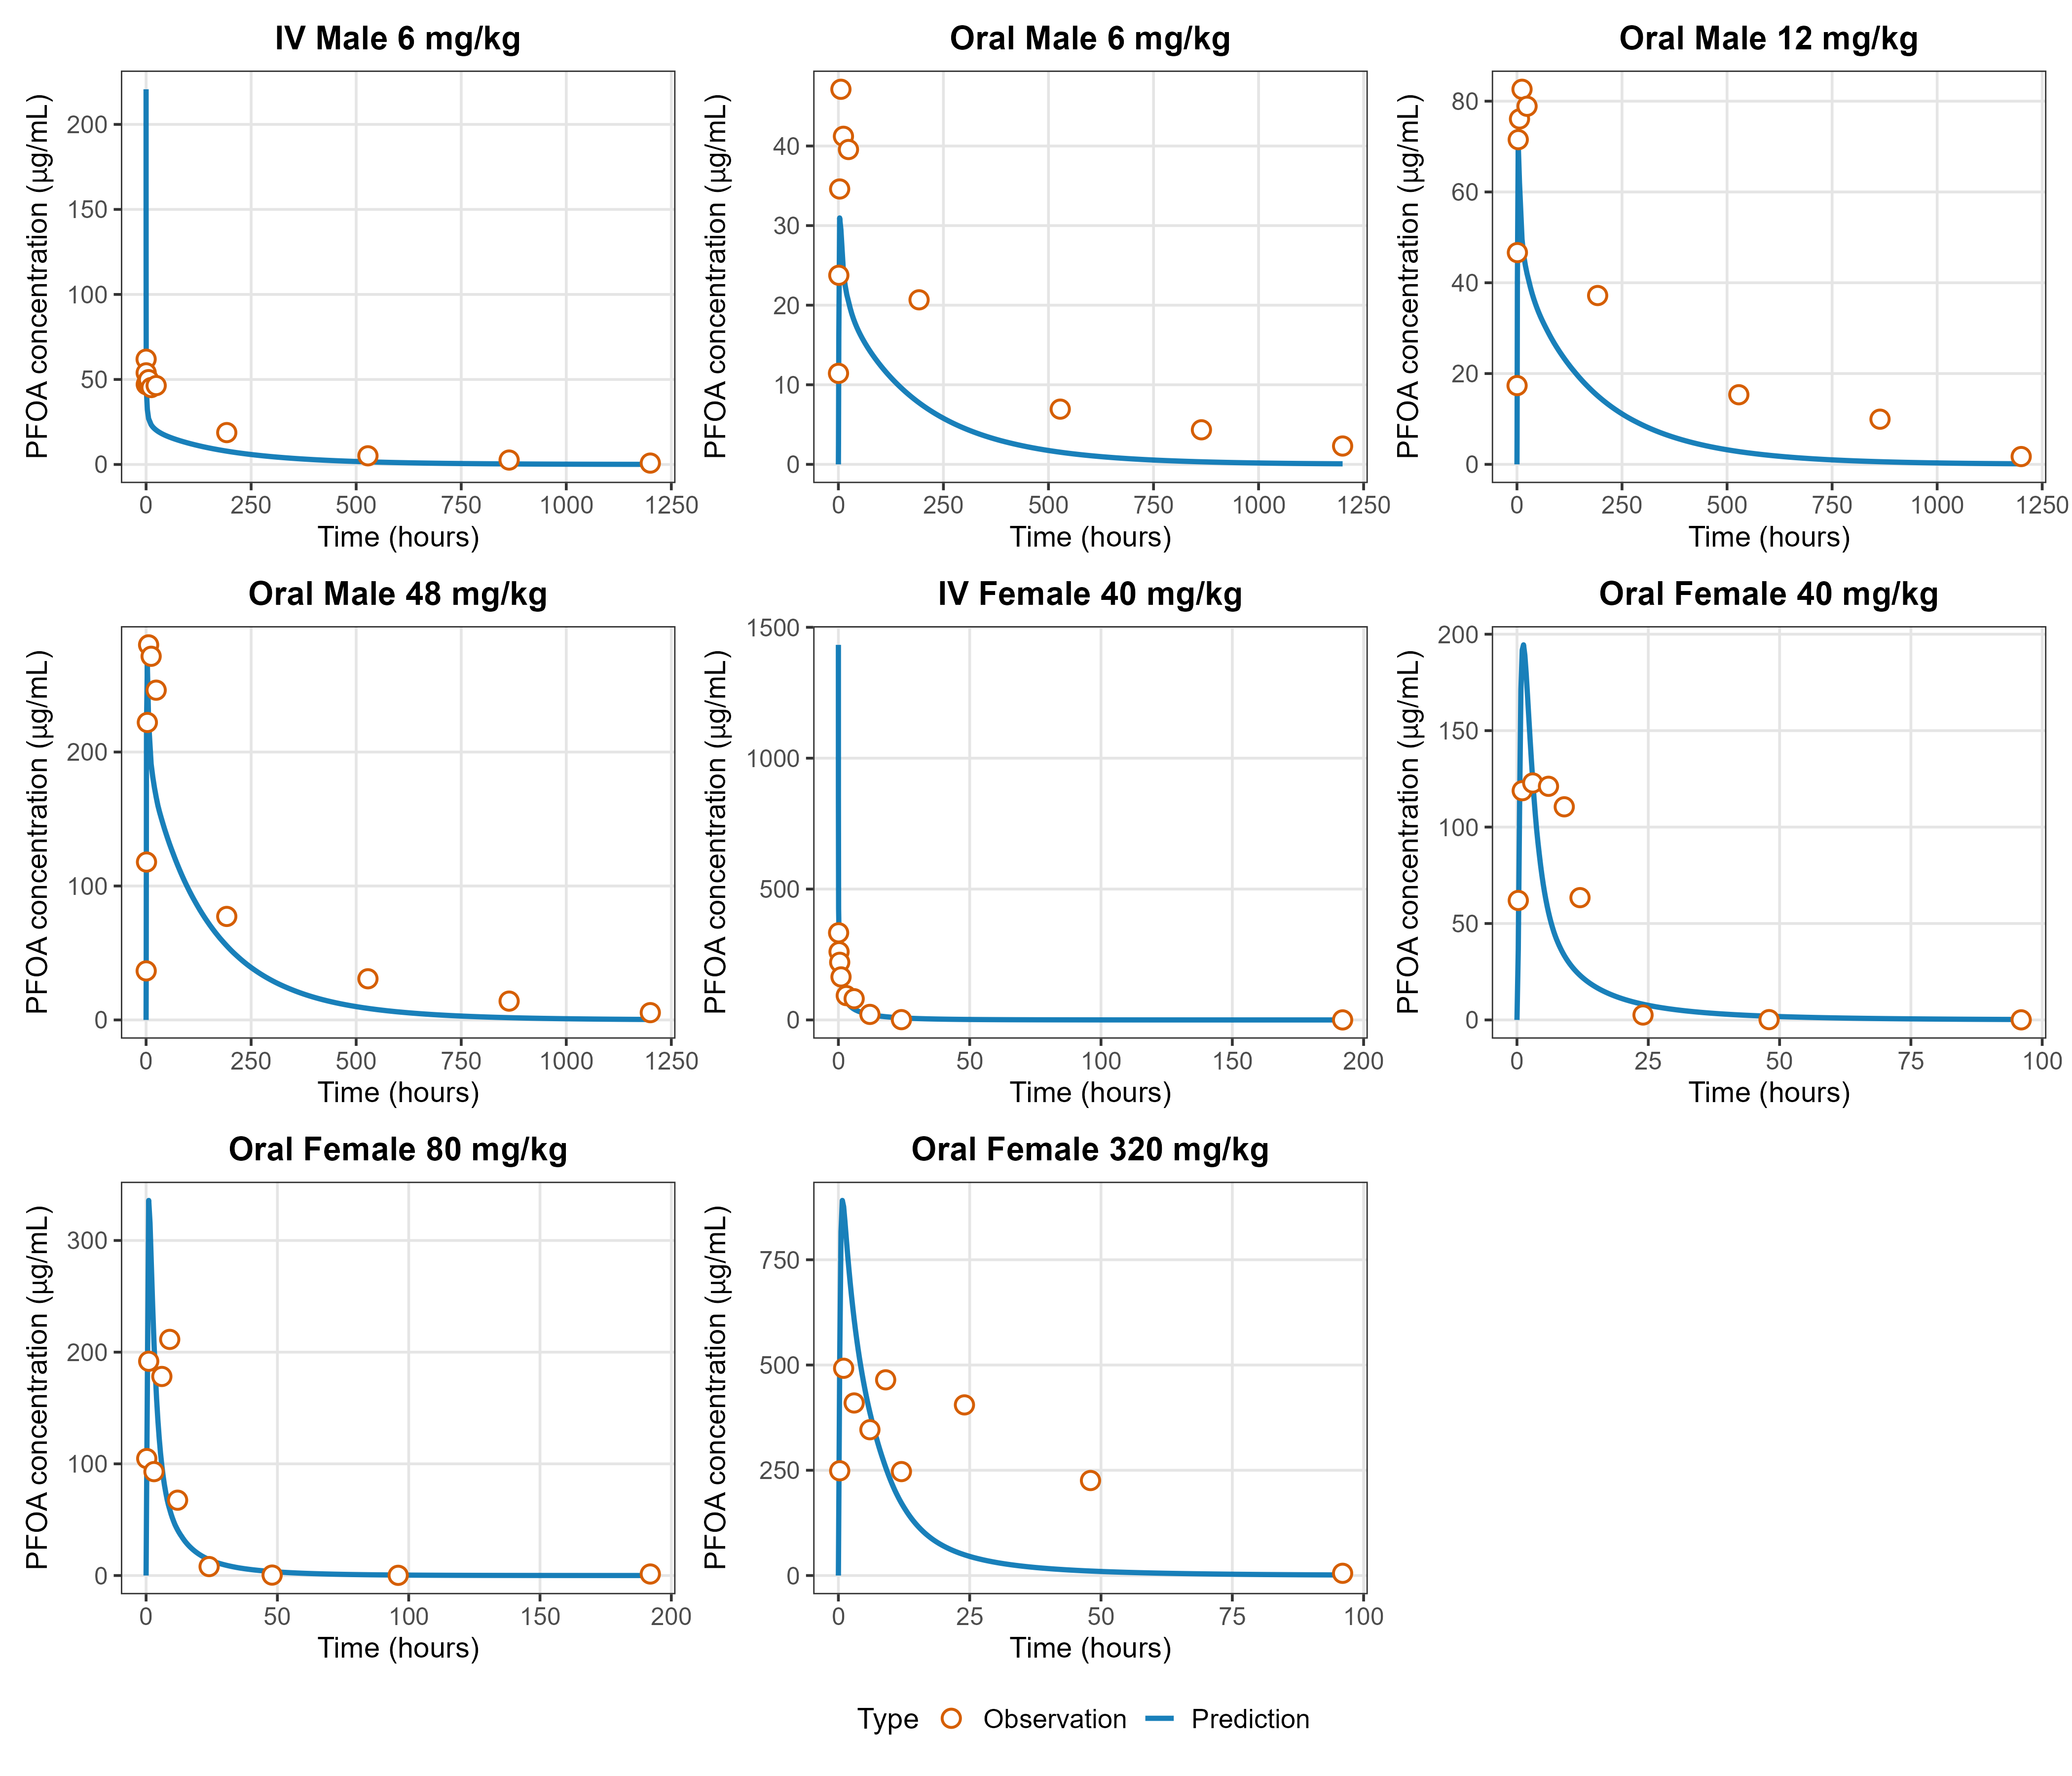
\includegraphics[width=1.0\textwidth]{Figures/serum_plots.png}
    \caption{Model predictions versus observed plasma concentrations following intravenous injection or oral ingestion in male and female rats. Applied doses were 6, 12, and 48 $mg/kg$ for males, and 40, 80, and 320 $mg/kg$ for females. Experimental data were obtained from \citet{dzierlenga_2020}. The average predictions $AAFE$ was 2.75}
    \label{fig:serum_gof}
\end{figure}



\begin{figure}[H]
    \centering
    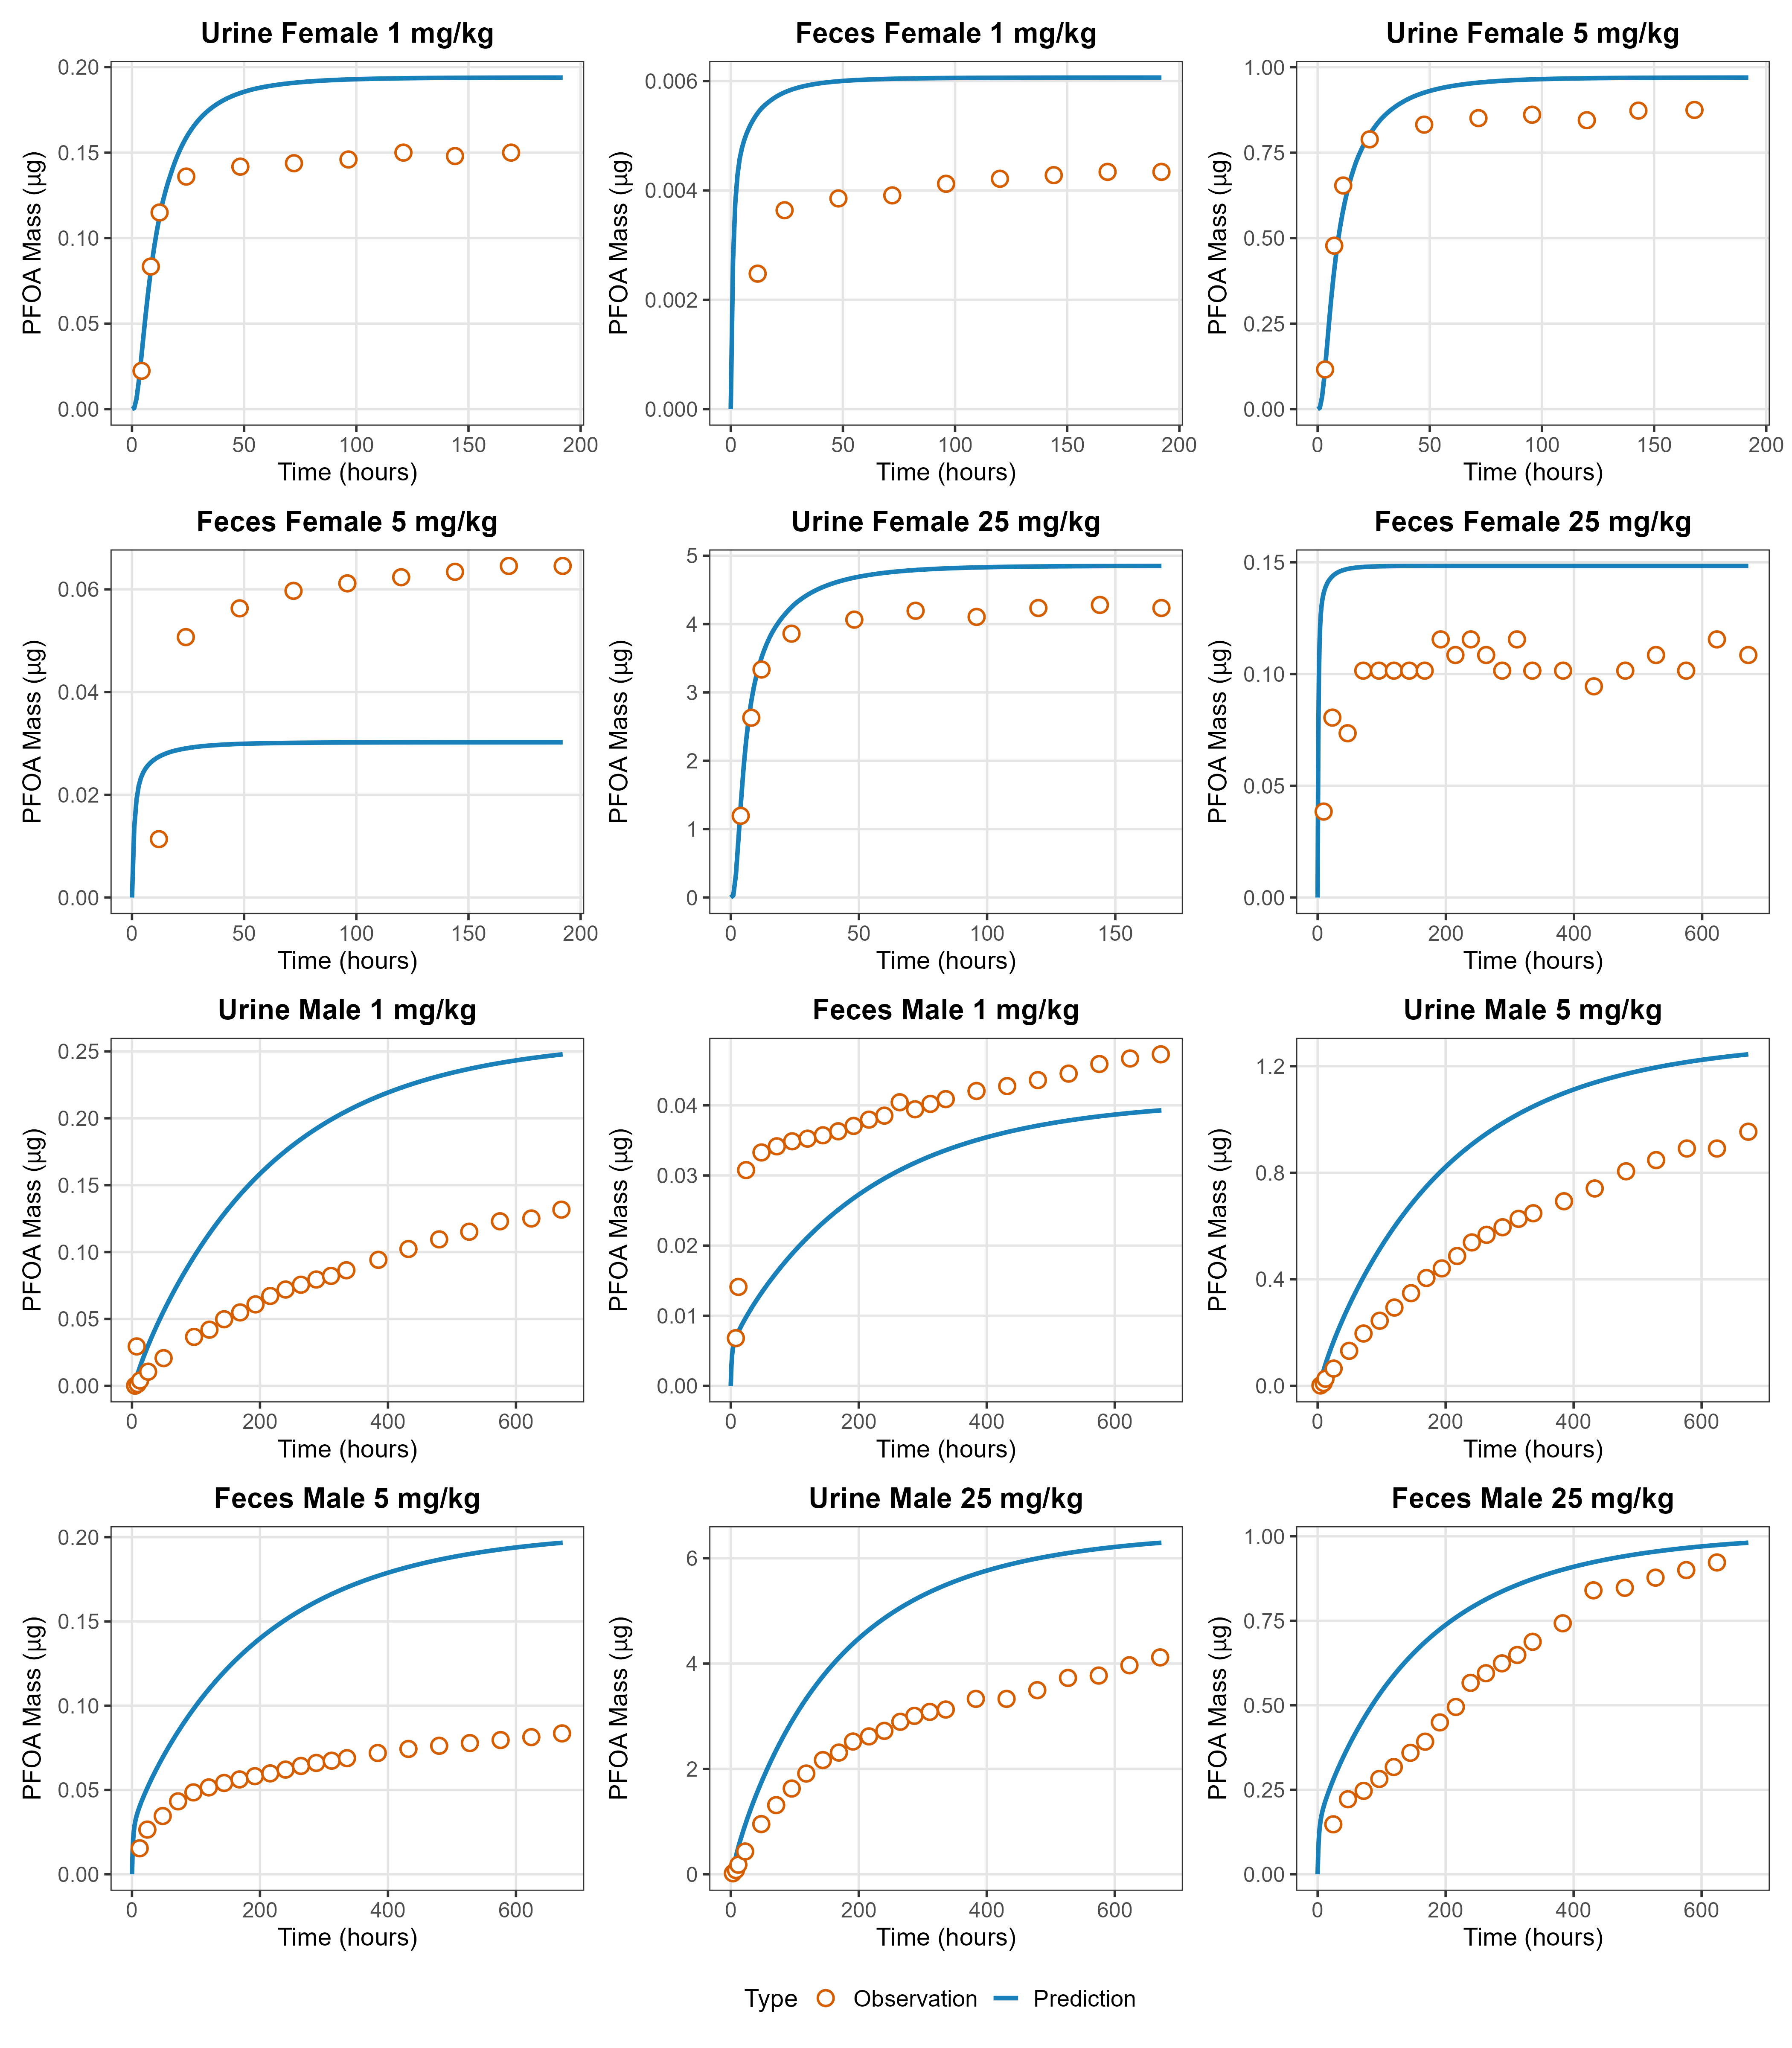
\includegraphics[width=1.0\textwidth]{Figures/excreta_plots.png}
    \caption{Model predictions versus observed cumulative PFOA mass in feces and urine following oral ingestion in male and female rats. Doses of 1, 5, and 25 $mg/kg$ were administered to both male and female rats. Experimental data were obtained from \citet{kemper_2003}. The average predictions $AAFE$ was 1.76}
    \label{fig:excreta_gof}
\end{figure}


 An essential component of ensuring model reliability is validation against independent datasets. In this study, the model was rigorously evaluated using data from five separate studies. Figure \ref{fig:validation} summarises the comparison between model predictions and experimental observations across the entire validation set. A quantitative overview is provided in Table \ref{Table:PFOA_validation}, showing that more than half of the data points fall within a two-fold error range, while nearly 90\% lie within three-fold, demonstrating the model’s capacity to capture PFOA dynamics across diverse administration scenarios. Study-specific validation plots are provided in Figures \ref{fig:validation_serum}–\ref{fig:validation_nasal}, with a detailed analysis of the AAFE for each study presented in Table \ref{Table:sup_validation_aafe}.

\begin{figure}[H]
    \centering
    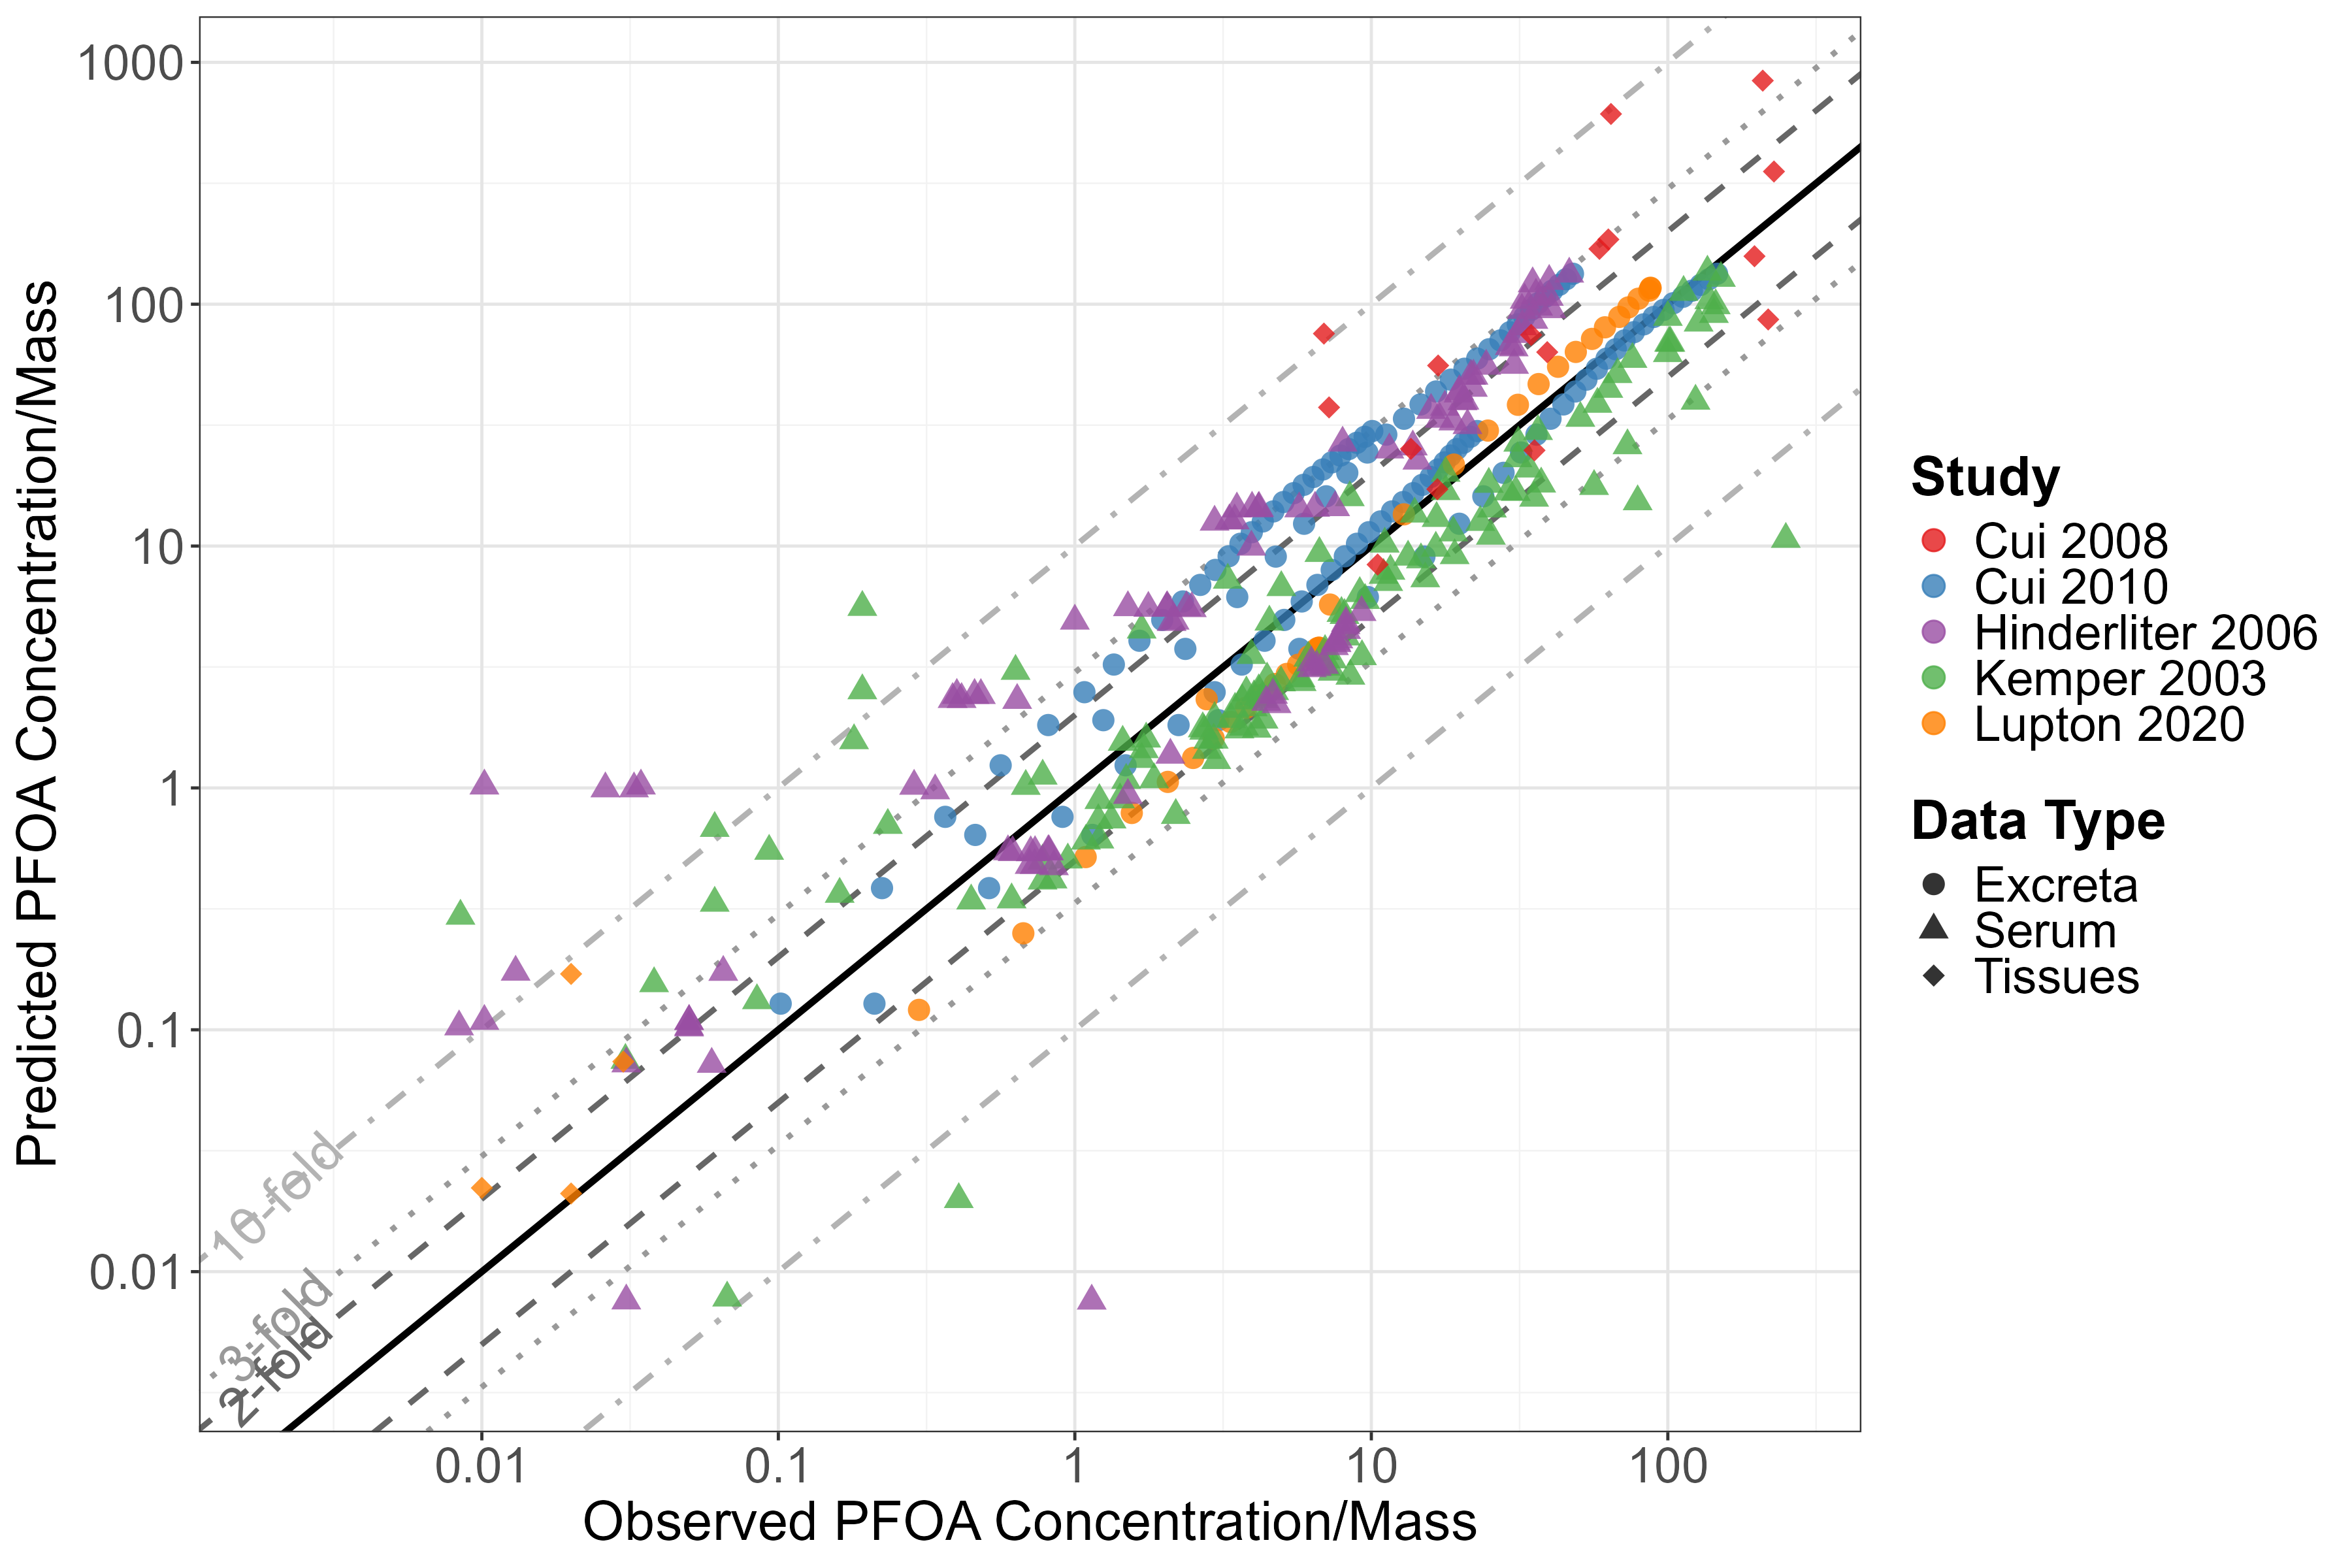
\includegraphics[width=1.0\textwidth]{Figures/validation.png}
    \caption{Model validation against data from \citet{cui_2009}, \citet{cui_2010}, \citet{lupton_2021}, \citet{hinderliter_2006}, and \citet{kemper_2003}. Predictions are compared with observations for excreta, serum, and tissues following oral or inhalation exposure, under single or repeated dosing in male and female rats.}
    \label{fig:validation}
\end{figure}

\begin{table}[h!]
\centering
\label{Table:PFOA_validation}
\caption{Overall model performance metrics on the validation dataset.}

\begin{tabular}{lccccc}
\hline
$n$ & RMSE& $AAFE$ &\% within 2-fold & \% within 3-fold & \% within 10-fold \\
\hline
395&  0.4305 & 2.10 & 56 & 85 & 96 \\
\hline
\end{tabular}
\end{table}
\newpage

Sensitivity analysis was performed to identify the most influential parameters across different organs. Results for male and female rats are presented as heatmaps in Figure \ref{fig:sensitivity}. The permeability coefficient between the renal tubule fluid and tubular cells, as well as between the intestinal lumen and enterocytes, was considered separately from the general cell permeability coefficient in order to highlight its specific contribution, even though the same numerical value was applied in the model. As shown in the figure, the albumin association constant emerged as the most influential parameter in both sexes, together with the permeability coefficient between interstitial and intracellular spaces, where both had a positive effect on nearly all organ AUCs. Oat1/3 transporters were also highly influential, with an increase in their relative activity factor (RAF) strongly decreasing the AUC of most organs. Conversely, increasing the permeability between renal tubule fluid and tubular cells elevated the AUC of all organs. Sex-specific effects were also observed. In males, an increase in Oatp RAF led to higher organ AUCs, whereas this effect was absent in females, as expected. Likewise, hepatic and fecal clearance had negligible impact in females, due to dominant renal elimination, but reduced organ AUCs in males. Increasing the hepatic Oatp RAF in males similarly enhanced fecal excretion. Binding of PFOA to L-FABP influenced only the liver in females, whereas in males it additionally reduced AUCs in other organs. Interestingly, paracellular permeability exhibited opposite effects between sexes. In males, increasing it elevated organ AUCs, whereas in females it reduced them. This behaviour reflects the greater amount transferred from kidney blood to the interstitial space, where PFOA can subsequently be translocated into the renal tubule through a combination of diffusion and active transport. As entirely expected, changes in the transcellular permeability coefficient had no measurable impact in either sex.


\begin{figure}[H]
    \centering
    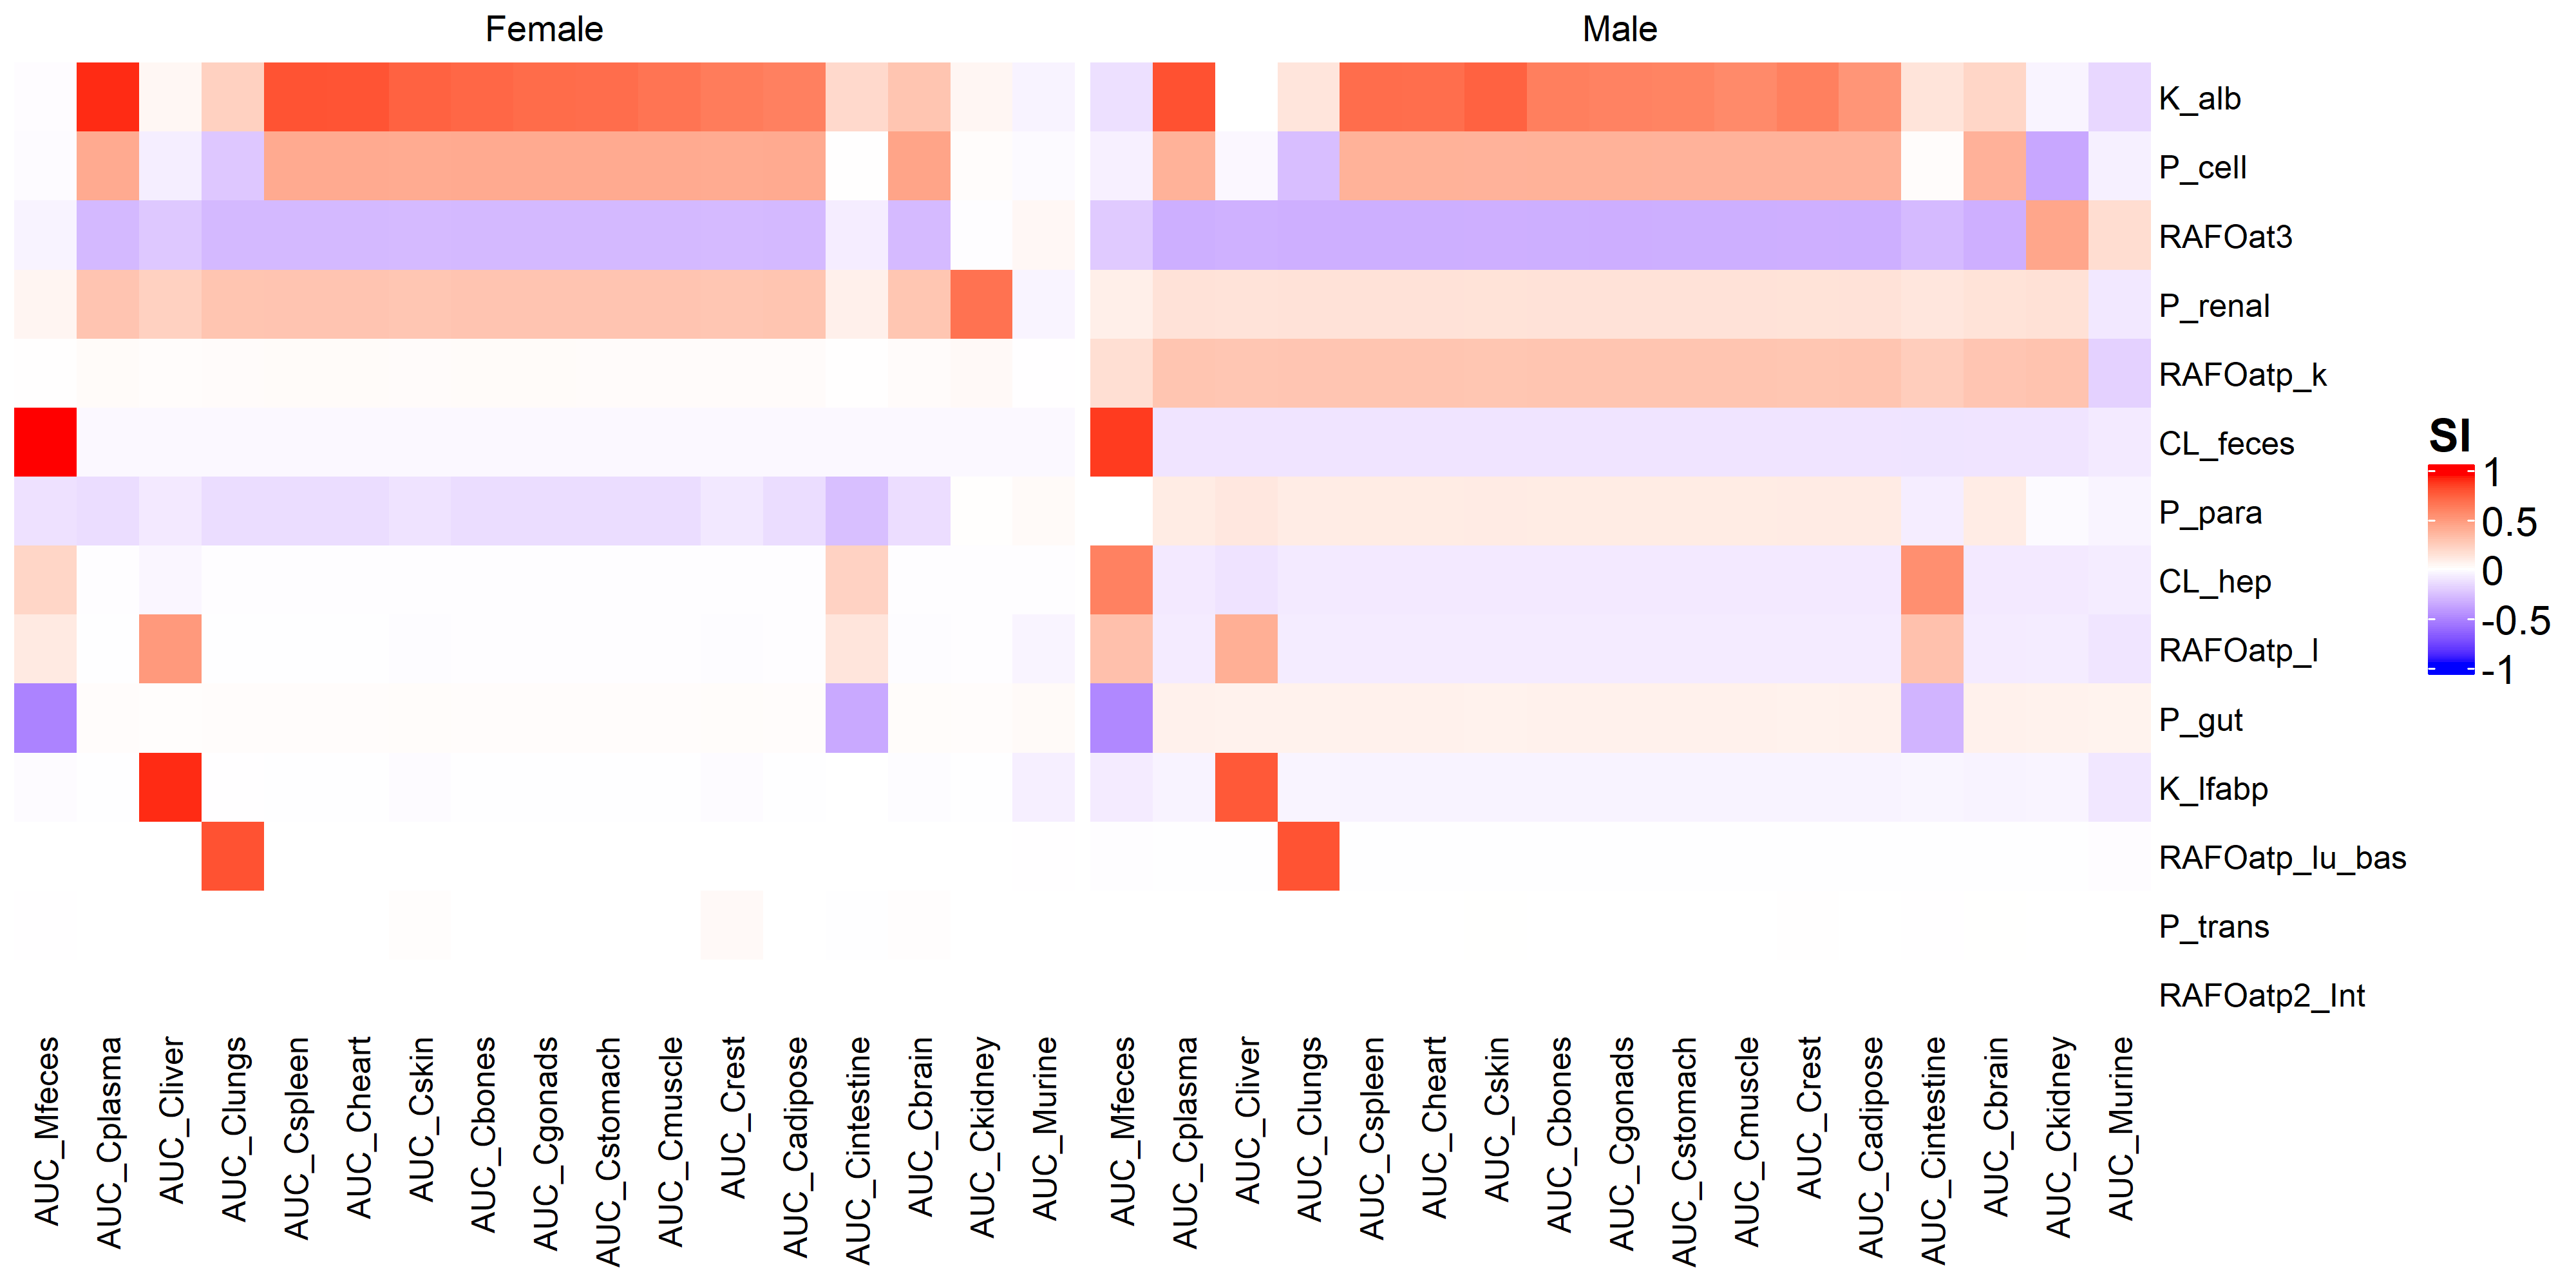
\includegraphics[width=1\textwidth]{Figures/sensitivity.png}
    \caption{Sensitivity analysis of key parameters in the male and female model. For both male and female rats, the baseline scenario simulated oral ingestion of 1 mg/kg PFOA. Colours are normalised to the overall minimum and maximum values across both sexes. The y-axis lists the parameters, and the x-axis represents the corresponding organ AUC. Parameters on the y-axis: $K\_alb$: albumin association constant, $P\_cell$: cell permeability coefficient, $RAFOat3$: RAF of renal Oat1/3, $P\_renal$: renal permeability coefficient, $RAFOatp\_k$: RAF of kidney Oatp1a1/Urat, $CL\_feces$: clearance to feces, $P\_para$: paracellular permeability, $CL\_hep$: hepatic clearance, $RAFOatp\_l$: RAF of liver Oatp1a1/Oatp2b1/Ntcp, $P\_gut$: permeability coefficient between intestinal lumen and enterocytes, $K\_lfabp$: binding affinity for L-FABP, $RAFOatp\_lu\_bas$: RAF of basolateral lung Oatp transporters, $P\_trans$: transcellular permeability coefficient, $RAFOatp2\_Int$: RAF of intestinal Oatp2b1 transporters.}
    \label{fig:sensitivity}
\end{figure}

An important component of the model that defines PFOA dynamics is membrane permeability. For transcellular permeability and cellular uptake, including uptake from the interstitial space, intestinal lumen, epithelial lining fluid, or renal tubular fluid, the permeability coefficient applied was set equal to the apparent permeability value reported by \citet{ryu_2024}. However, this value proved too low to capture the observed dynamics across different organs. To address this, we introduced an additional term representing paracellular diffusion from the vascular to the interstitial space. Details of the parameterisation of paracellular diffusion are provided in the Supplemental Information. As illustrated in Figure \ref{fig:permeability}, paracellular flux through capillary gaps was substantially greater than transcellular diffusion. For organs with continuous endothelium and tight junctions (e.g., lung and bone), the difference was modest. In contrast, for organs with fenestrated capillaries or sinusoidal structures (e.g., kidney and liver), paracellular transport exceeded transcellular flux by more than two orders of magnitude. For the brain, paracellular diffusion was disabled to account for the restrictive tight junctions of the blood–brain barrier. Notably, attempts to calibrate the model without including diffusion through capillary gaps, relying solely on the in vitro–derived transcellular permeability, resulted in very poor fits to the observed data (see Figure \ref{fig:paracellular}).

\begin{figure}[H]
    \centering
    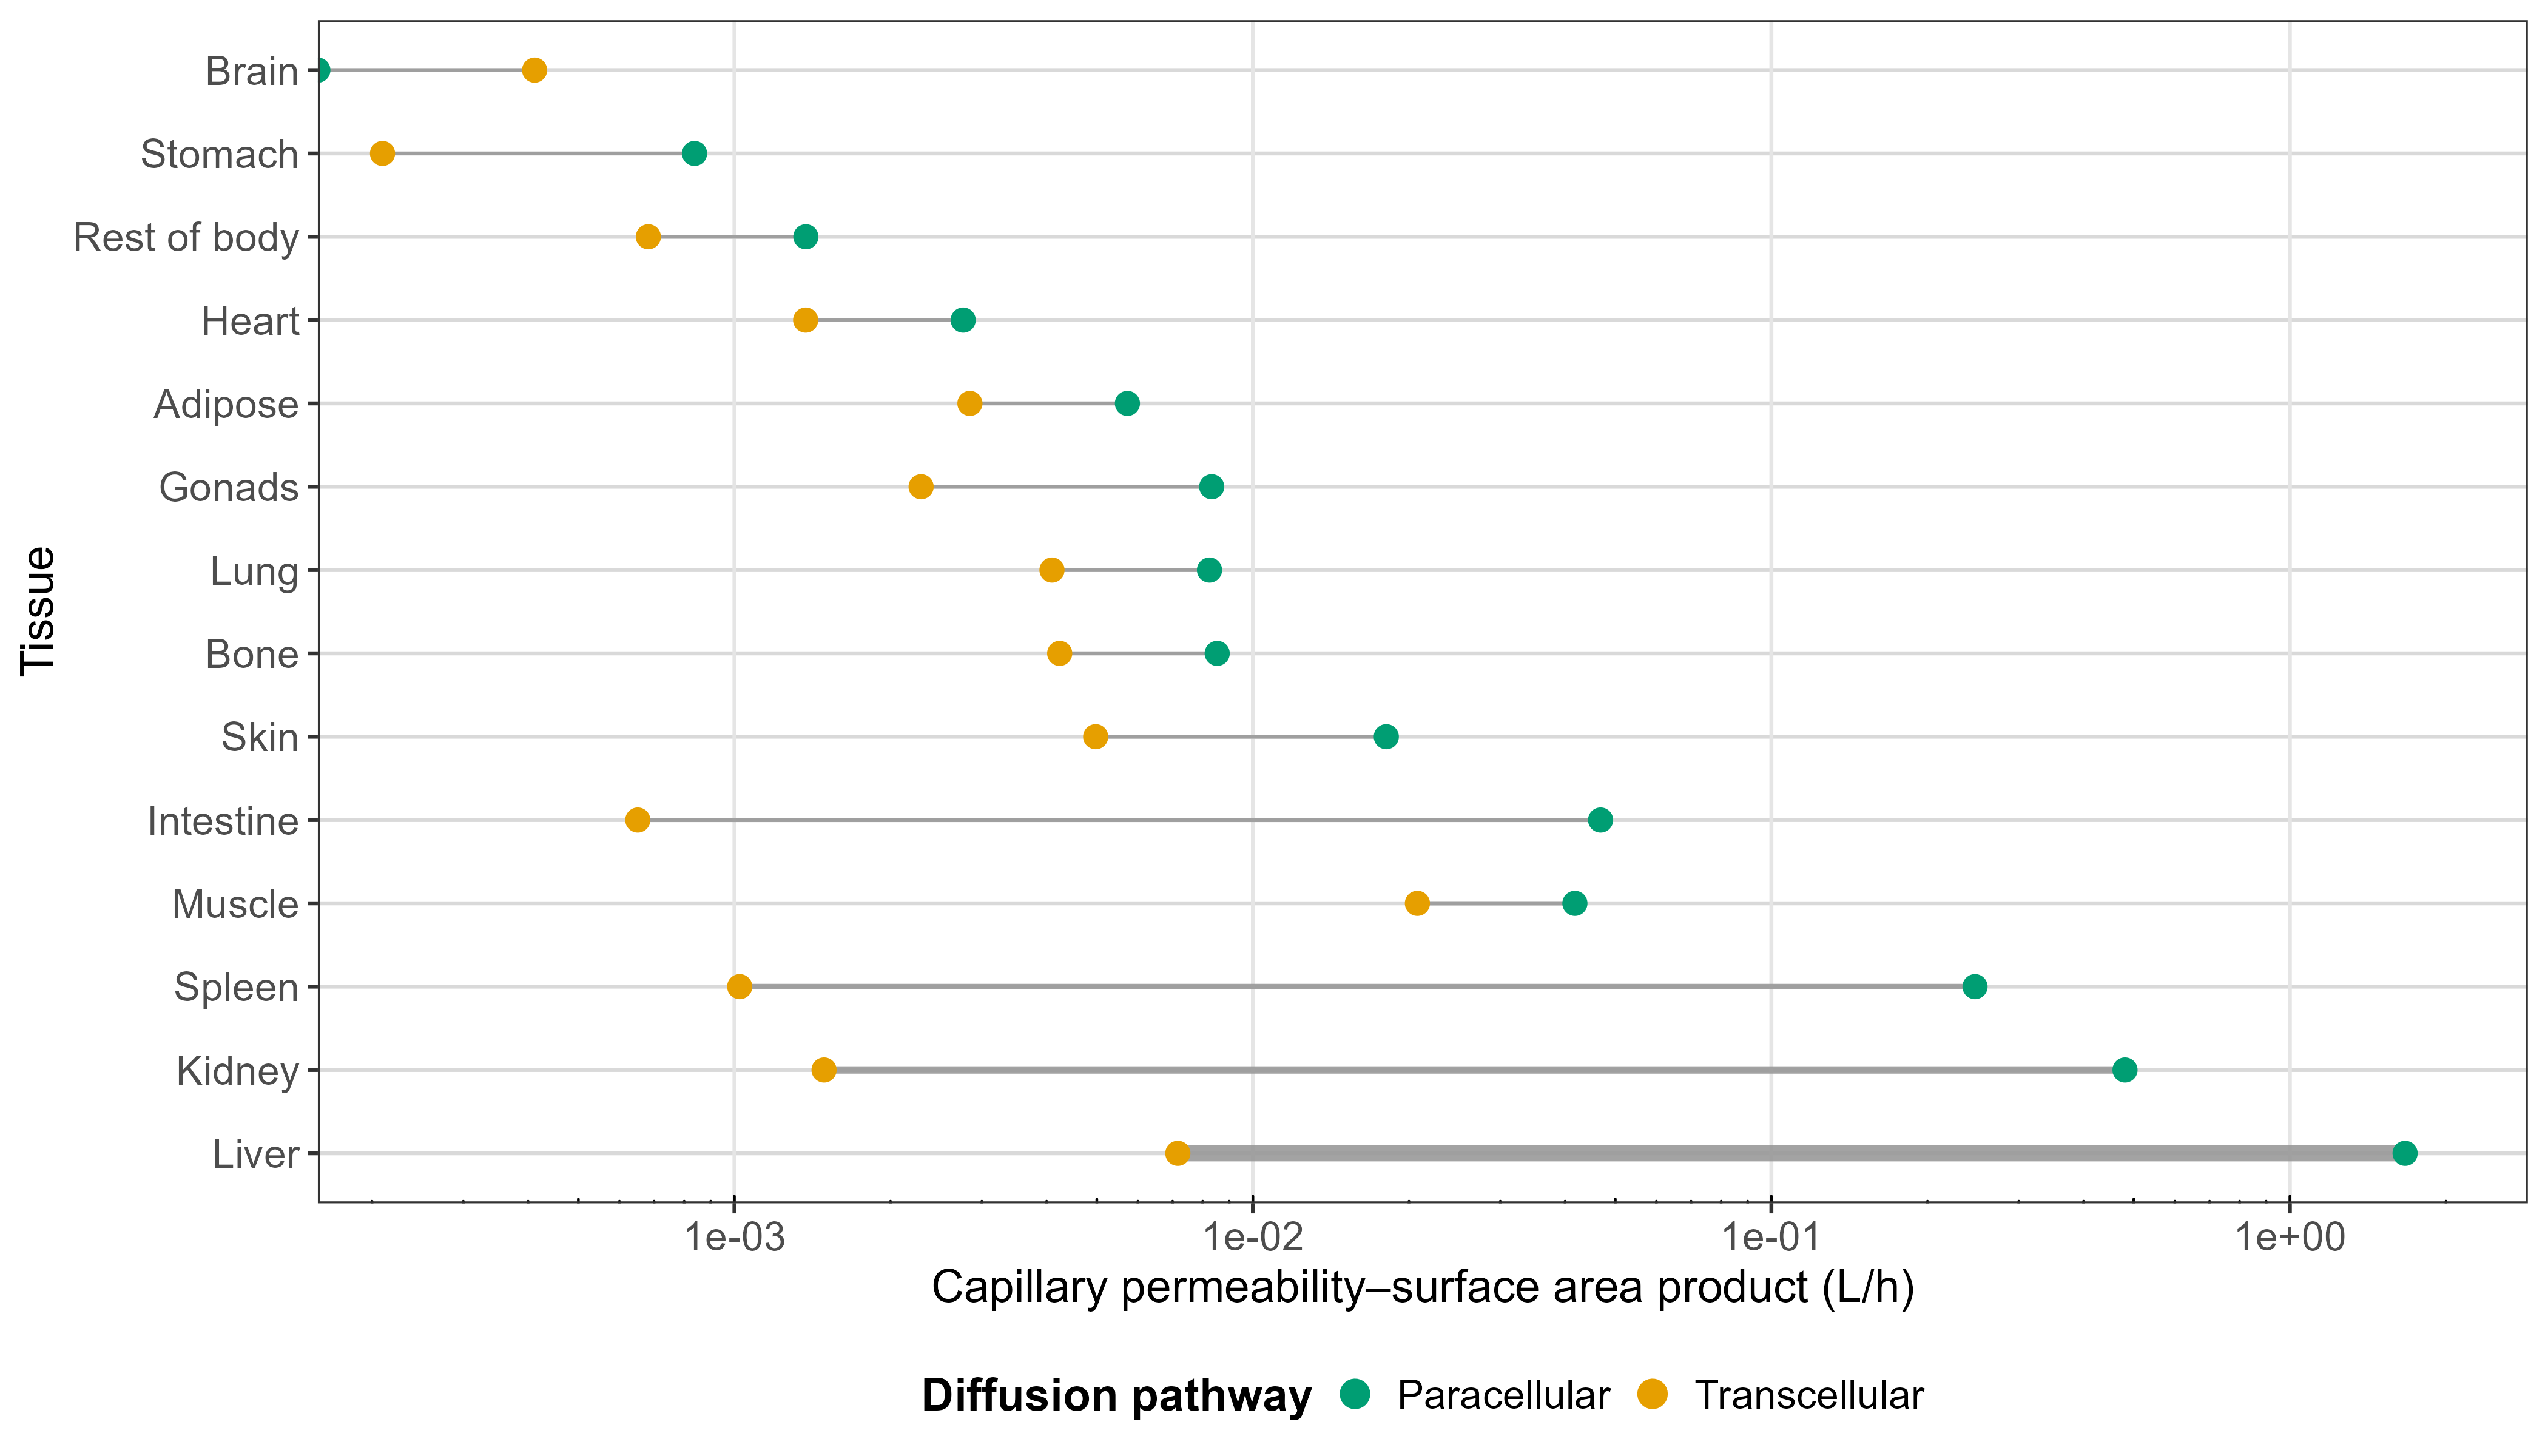
\includegraphics[width=1.0\textwidth]{Figures/permeability.png}
    \caption{ Simulated flux of PFOA from capillary blood to the interstitial space across all organs in a male rat administered 12 mg/kg PFOA. Yellow points indicate transcellular flux, while green points denote paracellular flux.}
    \label{fig:permeability}
\end{figure}

\noindent The model code is available at:\newline
\url{https://github.com/ntua-unit-of-control-and-informatics/multi-route-pbk-pfoa} \newline
The model can also be accessed as an easily accessible web application at:\newline
\url{https://jaqpot.org}


 

\section{Discussion}
\label{Discussion}

This study extended the mechanistic permeability-limited PBK model of \citet{cheng_2017} to female rats, testing whether the same mechanistic assumptions could also account for the rapid excretion observed in females. Sex-dependent parameterisation was applied, following the approach of \citet{worley_2015}, who, however, employed a simpler perfusion-limited model without detailed considerations of protein binding and transporter activity. In contrast, the model developed here relies primarily on physiological data, allowing safer extrapolation to humans through appropriate parameter scaling. Incorporating both diffusion and active transport in the permeability structure enabled the capture of PFOA dynamics, while protein binding alone was sufficient to reproduce tissue burden across species and doses. The model was parameterised using a middle-out approach, integrating both \textit{in vitro} and \textit{in vivo} data. The \textit{in vitro} values served as anchors, guiding parameter estimation towards physiologically plausible ranges for the fitted parameters. Overall, the model achieved a good fit to tissue concentration–time profiles without requiring any tissue-specific fitted parameters. Extended validation showed that the model consistently achieved very good predictive performance across a wide range of scenarios, encompassing multiple dose levels, both sexes, and various exposure routes. Finally, sensitivity analysis revealed that model predictions were most influenced by albumin binding, the relative activity factors of renal reabsorption and active secretion transporters, and cellular permeability. 

 


A key modelling decision in this study was the adoption of a permeability-limited framework. This choice was motivated by the physicochemical properties of PFOA, which is negatively charged at physiological pH, and its passage across membranes constitutes the rate-limiting step of distribution. Beyond \citet{cheng_2017}, several recent studies have also employed permeability-limited approaches to describe PFOA kinetics \citep{karakoltzidis_2025, choi_2024}. Notably, \citet{choi_2024} directly compared flow-limited and permeability-limited PBPK models across sexes and ages in rats, and extrapolated them to humans. They showed that both approaches could reproduce sex differences in rats. However, the permeability-limited model, informed by transporter kinetics and ontogeny, offered stronger mechanistic insight and yielded more reliable human predictions. In contrast, the simpler flow-limited model, when scaled allometrically, still provided a reasonable approximation of human PFOA disposition. Taken together with the findings of this study, the comparison suggests that permeability-limited models demand more effort and resources to develop but can provide deeper mechanistic explanations of observed patterns. By contrast, when human \textit{in vivo} data are available and the objective is to capture long-term equilibrium concentrations under chronic exposure, a perfusion-limited model may be sufficient. Nonetheless, when permeability is clearly the limiting step and short-term dynamics are of interest, a permeability-limited framework remains the most appropriate and informative choice.


Protein binding emerged as the most influential component of the model in both male and female rats. Binding was represented for three proteins, including albumin in blood and interstitial compartments, L-FABP in liver and kidney tissue, and A2U in male kidney tissue. The inclusion of A2U was primarily for completeness, as it did not affect model outcomes. Other binding interactions could also be considered. For example, \citet{fischer_2025} incorporated PFAS binding to phospholipids in a mouse PBK model and found it to be highly influential. In this study, a single binding site per protein was assumed, although multiple binding sites with different affinities would be more realistic. At high doses, non-specific binding may also become relevant. The initial free protein concentration in each compartment was set equal to the total protein concentration, although in reality it may be lower due to competition with endogenous ligands. Furthermore, the explicit binding kinetics implemented here were likely more detailed than necessary, since protein binding equilibrates much faster than PFOA distribution and can be reasonably treated as quasi-equilibrium. The main motivation for including these dynamics was to allow binding site saturation at high doses. For most scenarios, however, representing binding through the fraction unbound would be sufficient.



Including paracellular permeability was essential to accurately capture PFOA dynamics across tissues. This study is not the first to account for paracellular transport. For instance, \citet{korzekwa_2022} modelled diffusion through endothelial gaps using a parameter $P_{gap}$, assigning drug-specific low values scaled by $MW^{-3}$ to continuous capillaries and a single high value to fenestrated tissues. In the present work, paracellular diffusion was instead described by explicitly considering both the fraction of endothelial surface area covered by gaps and the organ-specific upper pore size limit. The authors recommend using Caco-2 or MDCK apparent permeability values to parameterise transcellular endothelial diffusion, as was also done in the present study. Without incorporating the paracellular pathway, reliance on an apparent \textit{in vitro} permeability estimate from an MDCK monolayer \citep{ryu_2024} resulted in unrealistically low permeation that could not reproduce observed data (Figure \ref{fig:paracellular}). However, this result should not be taken as direct proof of strong paracellular permeability for PFOA, as it may instead reflect the limited suitability of this assay for describing transcellular endothelial diffusion. Beyond capillary exchange, the same permeability values were applied to parameterise additional barriers, including intestinal absorption, renal tubular permeation, and generic cellular uptake. Permeability was assumed to be pH-independent within the range 5–8, consistent with \citet{ryu_2024}, who reported only minor differences between pH 6.5 and 7.4, likely due to the low pKa of PFOA.


Renal reabsorption of PFOA is the primary driver of its long half-life in humans \citep{worley_2017} and drives sex-dependent clearance in rats \citep{worley_2015}. For this reason, the kidney was represented in greater detail, incorporating segment-specific physiology such as localised transporter expression, segment volumes, surface areas, and flow reduction along the tubule. Figure \ref{fig:kidney_compartments} illustrates concentration changes along the renal tubule and within tubular cells, while Figure \ref{fig:flow_drop} shows how accounting for flow reduction along the nephron improves agreement with observed data. The representation of kidney interstitial space is particularly challenging. In this model, the interstitium was assumed to be uniformly distributed across the kidney, although in reality it is highly heterogeneous. For example, peritubular capillaries in the cortex lie in close proximity to proximal tubule cells, separated by an average distance of only 0.4 $\mu$m \citep{gazzard_2025}. According to \citet{lemley_1991}, approximately 26\% of the cortical tubular surface is in direct contact with peritubular capillaries, while 54–67\% is separated by a “narrow” interstitium accounting for just 0.6\% of total cortical volume. Blood supply is also region-specific. Proximal and distal convoluted tubules in the cortex are perfused by peritubular capillaries, whereas the medulla is supplied by the vasa recta. In the present model, all tubular cells are connected to a single interstitial space that directly communicates with capillaries. An alternative geometry that restricts peritubular capillary contact to cortical proximal and distal tubule cells may better reflect physiology. The large fitted value of Oat1/Oat3 RAF  observed here could, in part, be an artefact of these structural simplifications and the inherent complexity of nephron organisation.

A key limitation of this study is that animal variability was not explicitly encoded. The model was parameterised using data from rats of different ages, weights, and strains. In humans, the wide variability reported for PFOA half-life is thought to arise largely from differences in transporter protein expression. Similar differences likely exist in rats, contributing to heterogeneity in PK data. However, most available studies did not report individual data or measures of interindividual variability, making population modelling infeasible. Moreover, implementing a Bayesian population framework to fit such a large ODE system across multiple datasets would be computationally prohibitive. Even in the deterministic setting, parameter estimation proved challenging. Fixing many parameters to literature values helped reduce dimensionality, but fitting a large number of parameters remains difficult. Different algorithms, objective functions, and initial conditions were rigorously tested, yet given the complexity of the ODE system and data, there is no guarantee that the global optimum was reached.

\section{Conclusions}
This study provides a comprehensive evaluation of PFOA biodistribution in male and female rats through the development of a detailed permeability-limited PBK model. By integrating both \textit{in vitro} and \textit{in vivo} data across multiple exposure routes and dose levels, the model achieved reliable predictions that were supported by extensive validation. Sensitivity analysis highlighted the central role of albumin binding and renal transporter reabsorption in governing PFOA kinetics. This work demonstrates the value of mechanistic, physiology-driven modelling for improving understanding of PFOA biodistribution under diverse experimental conditions. Future studies should further refine kidney substructure to enhance physiological realism and continue probing the contribution of paracellular permeability, identified here as a key determinant of endothelial transport. Together, these advances can strengthen the predictive power of PBK models and support risk assessment efforts for PFOA and related PFAS.

\section*{Acknowledgements}
The authors acknowledge financial support by the SCENARIOS project
(Grant Agreement 101037509) which has
been funded by the European Commission under the Horizon
2020 Programme. 



\newpage

\bibliographystyle{apalike}  
\bibliography{Bibliography}
\end{document}


